% CS4246/5446 AY2627 S1 -- Final Report, version 2
% Single-column, 12pt, 1in margins. Figures and table bodies are produced by
% make_report_figures.py in this directory from saved run artifacts; figures in
% analysis/ come from the analysis scripts stored there.
\documentclass[12pt,a4paper]{article}

\usepackage[margin=1in]{geometry}
\usepackage[T1]{fontenc}
\usepackage{mathptmx}
% Times digits and letters in math; the symbol font stays Computer Modern because the
% Times-matched symbol font needs rsfs, which is not installed here.
\DeclareSymbolFont{symbols}{OMS}{cmsy}{m}{n}
\renewcommand{\ttdefault}{lmtt}
\usepackage{amsmath}
\usepackage{amssymb}
\usepackage{bm}
\usepackage{enumitem}
\usepackage{booktabs}
\usepackage{array}
\usepackage{tabularx}
\usepackage{longtable}
\usepackage{graphicx}
\usepackage[font=normalsize,labelfont=bf,skip=4pt]{caption}
\usepackage{float}
\usepackage{xcolor}
\usepackage{titlesec}
\usepackage{microtype}
\usepackage[hidelinks]{hyperref}

\graphicspath{{figures/}{analysis/}}

\titleformat{\section}{\normalfont\large\bfseries}{\thesection}{0.6em}{}
\titleformat{\subsection}{\normalfont\normalsize\bfseries}{\thesubsection}{0.6em}{}
\titleformat{\subsubsection}[runin]{\normalfont\normalsize\bfseries}{\thesubsubsection}{0.5em}{}[.]
\titlespacing{\section}{0pt}{10pt plus 2pt minus 2pt}{4pt}
\titlespacing{\subsection}{0pt}{8pt plus 2pt minus 2pt}{3pt}
\titlespacing{\subsubsection}{0pt}{6pt plus 2pt minus 2pt}{0.6em}
\titleformat{\paragraph}[runin]{\normalfont\normalsize\bfseries}{}{0pt}{}
\titlespacing{\paragraph}{0pt}{4pt plus 2pt minus 1pt}{0.5em}
\setlist{topsep=2pt,itemsep=1pt,parsep=0pt,leftmargin=*}
\setlength{\parskip}{4pt}
\setlength{\parindent}{0pt}
\setlength{\emergencystretch}{1.5em}
\setlength{\textfloatsep}{10pt plus 2pt minus 2pt}
\setlength{\floatsep}{8pt plus 2pt minus 2pt}
\setlength{\intextsep}{8pt plus 2pt minus 2pt}
\renewcommand{\topfraction}{0.85}
\renewcommand{\bottomfraction}{0.6}
\renewcommand{\textfraction}{0.12}
\renewcommand{\floatpagefraction}{0.75}
\renewcommand{\arraystretch}{1.1}

% Unit used in text and in math; in math it is set upright, not as a product of variables.
\DeclareRobustCommand{\bps}{\ifmmode\,\text{bps}\else\,bps\fi}
\newcommand{\todo}[1]{\fcolorbox{red!70!black}{red!6}{\parbox{\dimexpr\linewidth-2\fboxsep-2\fboxrule}{\textbf{TODO (team):} #1}}}
\newcommand{\gt}{\tilde g}
\newcommand{\bh}{\hat b}
\newcommand{\E}{\mathbb{E}}
\newcommand{\usd}[1]{\$#1}
% Table bodies are read with the primitive \input, which is expandable, so that
% \midrule and \bottomrule after an included body are still recognised.
\makeatletter
\newcommand{\tabinput}[1]{\@@input #1 }
\makeatother

\begin{document}
\pagenumbering{Alph}

% ------------------------------------------------------------------ title page
\begin{titlepage}
\centering
\vspace*{1.2cm}
{\large National University of Singapore \\ School of Computing \par}
\vspace{0.4cm}
{\large CS4246/5446 --- Reinforcement Learning and Sequential Decision Making \\
Semester 1, AY2026/27 \par}
\vspace{1.4cm}
{\LARGE\bfseries Final Report \par}
\vspace{0.3cm}
{\large Version 2: formal model, algorithm comparison and a basis-adjusted lead-lag agent \par}
\vspace{0.6cm}
{\Large Learning When \emph{Not} to Trade: Reinforcement Learning for \\[2pt]
Cross-Venue Latency Arbitrage After Transaction Costs \par}
\vspace{1.4cm}
{\large Group X \quad\textbar\quad Application Project \par}
\vspace{1.1cm}

\begin{tabular}{@{}lll@{}}
\toprule
\textbf{Name} & \textbf{Matriculation No.} & \textbf{Email} \\
\midrule
Kerk Tai Heng      & A0XXXXXXX & e1137106@u.nus.edu \\
$\langle$Member 2$\rangle$ & A0XXXXXXX & eXXXXXXX@u.nus.edu \\
$\langle$Member 3$\rangle$ & A0XXXXXXX & eXXXXXXX@u.nus.edu \\
$\langle$Member 4$\rangle$ & A0XXXXXXX & eXXXXXXX@u.nus.edu \\
$\langle$Member 5$\rangle$ & A0XXXXXXX & eXXXXXXX@u.nus.edu \\
$\langle$Member 6$\rangle$ & A0XXXXXXX & eXXXXXXX@u.nus.edu \\
\bottomrule
\end{tabular}

\vspace{0.8cm}
{\normalsize\textit{AI-use disclosure: AI coding agents (an OpenAI Codex-based agent and
Anthropic's Claude) implemented substantial parts of the software and drafted this report
under the team's direction. The full statement follows the conclusion.}\par}

\vfill
{\normalsize 6 October 2026 \par}
\end{titlepage}

\pagenumbering{arabic}
\setcounter{page}{1}

% ------------------------------------------------------------------ abstract
\phantomsection\label{bodystart}
\begin{center}{\large\bfseries Abstract}\end{center}
\vspace{-4pt}
We asked whether a reinforcement learning (RL) agent can trade Bitcoin perpetual futures
between Binance and Hyperliquid (HL) only when the price gap between the two venues pays for
fees, spread and execution delay. Version~1 of this report documented two agents trained with
proximal policy optimisation (PPO) that learned to stay flat. Version~2 states the task as a
semi-Markov decision process (SMDP) with
market dynamics that do not depend on the agent's actions, and uses that model to interpret
the failure: version~1 observed the raw gap, which mixes a slow price offset between the venues
(the basis) with a short-lived lead-lag component. On training days the raw gap had no gross
edge at any threshold from 1 to 10 basis points (bps). A causal 60-second moving average of
the gap, which serves as an approximate belief state for the basis, removed the offset; the
remaining de-meaned gap earned 2.91\bps{} gross per trade at a 3\bps{} threshold on the same
days. On this redesigned SMDP we compared PPO, a Double deep Q-network (Double DQN), fitted-Q
iteration (FQI) that treats the exit as an optimal-stopping problem, and a contextual-bandit
ablation without a learned exit; this comparison was registered after PPO's test results were
known. All were selected on validation days and tested once in the unchanged simulator with
fills 450\,ms after each decision. On four test days that earlier attempts had already
examined, PPO made \usd{76.91}, \usd{37.91}, \usd{2.21} and \usd{0.05} at taker fees of 0.5,
1, 2 and 3.5\bps{} per side, from 5,056 down to 45 trades; the last amount cannot be told
apart from zero. Paired hour-block bootstrap intervals put PPO ahead of Double DQN, FQI and
the bandit at 0.5 and 1\bps, level with the best hand-written rule (tuned on validation) at
0.5\bps{} and ahead of it at 1\bps{} (\usd{3.12}, 90\% interval \usd{0.80} to \usd{5.34}).
Double DQN beat PPO at 2\bps{} with 240 trades against 628. When fills were priced from HL's
own clock instead of the received book, profits survived only at 0.5\bps{} (PPO \usd{27.05}),
and even there the bandit lost money. These are simulated results on reused test days, and
they do not establish a deployable edge.

% ------------------------------------------------------------------ 1
\section{Introduction}\label{sec:intro}

\subsection{Problem}
Bitcoin perpetual futures (futures with no expiry date) trade on many venues at once, and a
price move does not reach every venue's order book at the same moment. A trader who sees a
move first on one venue can trade on a venue whose quotes have not yet adjusted and exit when
the two prices converge. This is latency arbitrage. Budish, Cramton and Shim~\cite{budish}
describe the same mechanism in equity markets.

An order book lists resting buy orders (bids) and sell orders (asks). The mid price is the
average of the best bid and the best ask, and the spread is their difference. We measure the
gap as the Binance mid minus the HL mid, divided by the HL mid, in basis points (bps; 1\bps{}
is 0.01\%). An order that executes immediately against resting orders is a taker order: it
buys at the ask, sells at the bid and pays a taker fee on every fill. ``Per side'' means per
fill. A round trip therefore costs two fees, about one HL spread (median 0.12\bps) and any
slippage, an execution price worse than the quoted one (0.1\bps{} per fill in our model). At
1\bps{} per side the round trip costs about 2.3\bps; at 3.5\bps{} per side about 7.3\bps.

The question was whether an RL agent can learn from recorded order books to enter only when
the expected convergence covers these costs, exit at the right time, and do better than
hand-written rules under identical costs on later days. The proposal named proximal policy
optimisation (PPO)~\cite{ppo} as the main method and a deep Q-network (DQN)~\cite{dqn} as a
value-based comparison.

\subsection{What changed since version 1}
Version~1 trained two PPO designs. Both ended with zero validation trades, and the selected
policy of the first made zero trades on the test days, while a fixed 10\bps{} threshold rule
made \usd{1.19} over 16 trades at 3.5\bps{} per side. Version~2 changed the problem
formulation, the signal, the evaluation protocol and the set of algorithms:
\begin{itemize}
\item The task is written as an SMDP with a factored state, state-dependent action sets and
exogenous market dynamics (Section~\ref{sec:smdp}). Version~1 is recast as a partially
observable problem with a hidden basis (Section~\ref{sec:pomdp}).
\item The signal is the gap minus a causal estimate of the basis. The agent is consulted only
at seconds where this de-meaned gap is at least 2\bps{} and at every second while it holds a
position, and the fee is part of the state, so one network serves every fee level.
\item The primary fill delay is 450\,ms after the decision instead of 150\,ms, because HL's
book reaches the recorder about 340\,ms after HL's own timestamp
(Section~\ref{sec:filltiming}).
\item A protocol registered before any validation result fixed the splits, the candidate runs
and the selection rule. Five dated amendments followed; the one that made the 450\,ms group
primary and set the paired endpoint came after partial test results had been seen, and the one
that added the new algorithms came after all PPO test results (Section~\ref{sec:protocol}).
\item Double DQN~\cite{ddqn}, fitted-Q iteration~\cite{ernst,nfq} and a contextual-bandit
ablation (a one-step learner that only decides whether to enter) were trained on the same SMDP
and compared with PPO and with hand-written rules (Section~\ref{sec:algos}).
\end{itemize}

\subsection{Contributions}
\begin{enumerate}
\item A formal SMDP model of the task in which the market evolves independently of a
0.001\,BTC order. Under that assumption, and given the simulator's fill model, any policy's
return on recorded data follows by replay without policy-induced distribution shift, the exit
is an optimal-stopping problem, and the entry is close to a contextual bandit. These
consequences shaped the choice of algorithms.
\item A diagnosis of version~1's abstention that is consistent with the training data: on
training days, entering on the raw gap lost money before fees at every threshold from 1 to
10\bps, so abstaining was a reasonable response to that observation. We did not run an
ablation that isolates this cause.
\item A version~2 agent that trades. On the four test days, which were examined before, PPO's
net profit after modelled costs was positive at 0.5, 1 and 2\bps{} per side and could not be
told apart from zero at 3.5\bps, with fills 450\,ms after the decision. Under the stricter
HL-clock fill convention it was positive only at 0.5\bps{} per side.
\item A comparison of four learners, registered before the three new ones were trained but
after the PPO test results were known. PPO was conclusively ahead of Double
DQN, FQI and the bandit at 0.5 and 1\bps{} per side, tied the best hand-written rule
at 0.5\bps{} and beat it at 1\bps. Double DQN beat PPO at 2\bps.
\item An analysis of sub-second data that estimates, conditional on the HL-clock convention,
how much faster feeds would add, with numbers for each source of delay.
\end{enumerate}

% ------------------------------------------------------------------ 2
\section{Data}\label{sec:data}
The team recorded both venues' public order-book streams into one ClickHouse table: Binance
\texttt{btcusdt@depth20@100ms} (20 levels per side, 9.32 snapshots per second on average) and
HL \texttt{l2Book} (5 levels per side, 1.84 snapshots per second). The research range is the
30 complete days from 3 September to 2 October 2026 (UTC), 28,917,283 raw rows,
split by date into 22 training, 4 validation and 4 test days (Table~\ref{tab:data}). We call
the test days of 29 September to 2 October test~A; the day of 3 October, prepared separately,
is test~B. The data are public market feeds and contain no personal information.

Decisions are made on whole UTC seconds. Every row takes, for each venue, the latest snapshot
received at or before its timestamp, so no row uses information that arrived later. Version~2
adds execution rows at 150, 300, 450 and 600\,ms after each decision second (version~1 had 150
and 300\,ms). Five-minute windows with any invalid row (stale or missing quotes, crossed
books) are dropped whole; the extra offsets add quality checks, so 8,227 windows are kept
instead of version~1's 8,245: 5,970 training, 1,117 validation and 1,140 test windows, plus
285 on 3 October. At decision rows the median HL quote age (row time minus HL's exchange
timestamp) was 623 to 640\,ms; the median top-of-book spread was 0.012\bps{} on Binance and
0.12\bps{} on HL.

\begin{table}[!htbp]
\centering
\caption{Splits. Window counts are version~2's. Gap statistics are version~1's, computed on
its slightly larger set of windows (5,984, 1,121, 1,140 and 286); gap is
$10^4\times(\text{Binance mid} - \text{HL mid})/\text{HL mid}$.}
\label{tab:data}
\small
\begin{tabular}{@{}llrrrr@{}}
\toprule
 & & Windows & \multicolumn{2}{c}{$|$gap$|$ (bps)} & Seconds with \\
\cmidrule(lr){4-5}
Split & Dates (2026) & (version 2) & Median & p99 & $|$gap$|\geq 7$\bps{} \\
\midrule
Train      & 3--24 Sep     & 5,970 & 1.34 & 12.57 & 18.04\% \\
Validation & 25--28 Sep    & 1,117 & 1.30 &  5.20 & 0.084\% \\
Test A     & 29 Sep--2 Oct & 1,140 & 1.04 &  4.86 & 0.097\% \\
Test B     & 3 Oct         &   285 & 0.61 &  2.31 & 0.0047\% \\
\bottomrule
\end{tabular}
\end{table}

The training split has far more large gaps than the later splits. From 18 to 23 September
the Binance mid sat below the HL mid for whole days, with daily median signed gaps between
$-2.4$ and $-9.8$\bps, and these six days held 99.7\% of the training seconds with an
absolute gap of 7\bps{} or more. On those days the large gaps came from a slow, persistent
offset between the venues (a basis). Perpetual futures are tied to the spot price by
funding payments between long and short holders, and a funding difference between venues can
sustain such an offset; funding rates are not in the source table, so we could not test this.
This offset is why the raw gap had no edge on training days (Section~\ref{sec:why}).

% ------------------------------------------------------------------ 3
\section{Environment and execution model}\label{sec:env}

\subsection{Replay and costs}
Test results for the frozen choices in the main tables come from version~1's simulator,
unchanged; it follows the Gymnasium interface~\cite{gym}. An order decided at second $t$ fills
at the replay row $L$\,ms later. A fill walks the far side of the recorded HL book for the
order size and pays the volume-weighted average price (VWAP) over the levels it consumes,
moved 0.1\bps{} against the trader as slippage; a taker fee is charged on the fill notional
(price times quantity). An entry is rejected if HL's quote age or receive age (row time minus
the time the recorder received the book) exceeds 1,000\,ms at the decision or at the fill.
Positions are 0.001\,BTC (about \usd{84}), at most one at a time, closed by force 30\,s after
the entry fill or at the window's last row. Table~\ref{tab:env} lists the settings.

The simulator steps one second at a time and runs at about 3,500 steps per second, too slow
for many passes of PPO over 22 days. Training, validation selection, the stress tests, the
HL-clock fills and the same-snapshot split of Section~\ref{sec:stress} therefore use a fast
replay over a precomputed per-second table that runs about 1,500 PPO steps per second per
process. Unit tests check that it reproduces the simulator trade for trade for rule policies
at all four latencies, including forced exits, and the selected PPO policies gave the same
trade counts and the same test P\&L to the cent in both (Tables~\ref{tab:test450}
and~\ref{tab:ppo_runs}). The HL-clock
convention has no counterpart in the simulator, so no such check covers it.

\begin{table}[!htbp]
\centering
\caption{Execution settings shared by every policy in version~2.}
\label{tab:env}
\small
\begin{tabular}{@{}lr@{}}
\toprule
Parameter & Value \\
\midrule
Taker fee per side, evaluation & 0.5, 1, 2, 3.5\bps{} (4.5\bps{} stress) \\
Taker fee per side, training (sampled per window) & 0.5, 1.0, \ldots, 3.5\bps{} \\
Fill latency after the decision second & 450\,ms; 150\,ms (sensitivity); 300, 600\,ms (stress) \\
Slippage per fill & 0.1\bps \\
Spread multiplier & 1.0 (1.5 as a stress test) \\
Position size & 0.001\,BTC, one position at a time \\
Maximum holding time & 30\,s from the entry fill \\
Entry freshness limit (quote and receive age) & 1,000\,ms \\
Reference capital & \usd{10,000}, reset each window \\
Funding & not available; set to zero \\
\bottomrule
\end{tabular}
\end{table}

\subsection{Fill-timing conventions and why they matter}\label{sec:filltiming}
The simulator prices a fill at $t+L$ from the latest HL book \emph{received} by the recorder at
or before $t+L$. Two facts make this optimistic. First, HL's book arrives late: on six
training days the receive time minus HL's exchange timestamp had a median of 338\,ms
(10th to 90th percentile 304 to 429\,ms; this includes any clock offset between the machines).
Second, HL publishes a new book only every 540\,ms at the median. A fill priced at
$t+150$\,ms from the received book therefore often uses the same snapshot the decision already
saw, a price that was known before the order was sent: 71\% of the frozen 450\,ms PPO
policy's test entries did so when replayed with 150\,ms fills (Table~\ref{tab:samesnap}).

We therefore used three conventions. \emph{Received book} is the simulator's. \emph{HL clock}
prices the fill from the last HL book whose exchange timestamp is at or before $t+L$, which
assumes our clock matches HL's. \emph{Next snapshot}, used only in the sub-second analysis,
takes the first HL book stamped after $t+L$. On the six training days, entering at a
de-meaned gap of 3\bps{} or more and exiting 3\,s later earned 3.39\bps{} gross per trade
with received-book fills at 150\,ms, 2.04\bps{} with HL-clock fills and 0.63\bps{} with
next-snapshot fills. A received-book fill at 450\,ms approximates a 150\,ms order delay plus
HL's publication lag, so the 450\,ms group is primary and HL-clock fills are a stress test.
The HL-clock stress at $L=450$\,ms assumes that the order reaches HL 450\,ms after the
decision on HL's own clock. It therefore combines a 450\,ms order path with HL's publication
lag and is roughly a received-book fill 790\,ms after the decision (450 plus the 338\,ms
median lag). The HL-clock convention that matches a 150\,ms order delay is HL clock at
150\,ms, whose 2.04\bps{} on the six days is close to the 2.05\bps{} that received-book fills
at 450\,ms earned on all 22 training days (Section~\ref{sec:why}).

% ------------------------------------------------------------------ 4
\section{Formal problem: a semi-Markov decision process}\label{sec:smdp}

\subsection{Episodes and decision epochs}
Each retained five-minute window is one finite-horizon episode with whole seconds
$t\in\{0,\ldots,299\}$. The agent is consulted only at decision epochs
$0\leq t_0<t_1<\cdots<t_K\leq 299$, a subset of seconds that depends on the market path and
on the agent's position. Between epochs the position stays as it is. Because the sojourn time
$\tau_k=t_{k+1}-t_k$ varies, the process is a semi-Markov decision process: in the options
framework of Sutton, Precup and Singh~\cite{options}, ``stay as you are until the next epoch''
is a fixed option whose duration depends on the state. Figure~\ref{fig:smdp} shows the two
position phases.

\begin{figure}[!htbp]
\centering
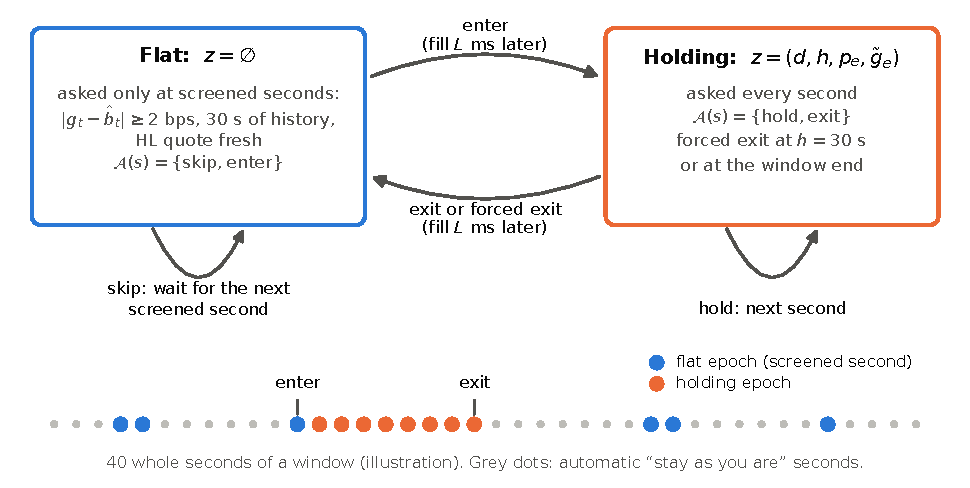
\includegraphics[width=\textwidth]{fig_smdp.pdf}
\caption{The decision process. A flat agent is asked only at screened seconds; a holding
agent is asked every second. Orders fill $L$\,ms after the decision. The timeline below is an
illustration of how epochs fall within a window, not data.}
\label{fig:smdp}
\end{figure}

\subsection{State}
The state at epoch $k$ factorises as
\begin{equation}
s_k=(x_{t_k},\,z_k,\,f).
\label{eq:state}
\end{equation}
The \emph{market state} $x_t$ holds what the recorded books show at second $t$: the gap
$g_t=10^4(m^{B}_t-m^{H}_t)/m^{H}_t$, where $m^B_t$ and $m^H_t$ are the Binance and HL mids;
the basis estimate $\bh_t$ and the de-meaned gap $\gt_t=g_t-\bh_t$; 1\,s and 5\,s mid returns
on both venues; the 30\,s realised volatility (standard deviation) of Binance's 1\,s returns;
the HL spread; HL's quote age and receive age; the order-book imbalance on each venue, (bid
volume $-$ ask volume)/(total volume) over the displayed levels; the time left in the window; and the length of uninterrupted history $n_t$. The basis estimate is an exponential
moving average (EMA) of earlier gaps,
\begin{equation}
\bh_t=(1-\alpha)\,\bh_{t-1}+\alpha\,g_{t-1},\qquad \alpha=\tfrac{2}{61},
\label{eq:ema}
\end{equation}
a 60-second span that excludes the current second and restarts wherever retained windows
are not adjacent.

The \emph{position state} is $z=\varnothing$ when flat and $z=(d,h,p_e,\gt_e)$ when holding,
with direction $d\in\{-1,+1\}$ ($+1$ is long HL), holding time $h$ in seconds, entry fill price
$p_e$ and the de-meaned gap at entry $\gt_e$. The fee $f$ per side is fixed within an episode
and drawn per training window from $\mathcal{F}_{\text{train}}=\{0.5,1.0,\ldots,3.5\}$\bps.
The agent observes $f$, so the task is an ordinary MDP whose state is augmented with an
episode-constant fee, and one policy $\pi(a\mid x,z,f)$ serves every fee. This differs from
the contextual MDPs of Hallak et al.~\cite{cmdp}, where the context is hidden.

The network sees a 20-dimensional observation $o=\psi(x,z,f)$ of the state~\eqref{eq:state}:
an in-position flag, the direction-signed market features, the fee, holding time, unrealised profit at the decision
row's exit price, $\gt_e$, time left and history length. Signed features are multiplied by
the trade direction ($\operatorname{sign}\gt_t$ when flat, $d$ when holding), so the network
does not have to learn the long and short cases separately. Every feature is divided by a
fixed constant and clipped to $[-10,10]$; no scale is fitted to any split.

\subsection{Actions}
The action set depends on the state:
\begin{equation}
\mathcal{A}(s)=\begin{cases}\{\text{skip},\ \text{enter}\} & z=\varnothing,\\
\{\text{hold},\ \text{exit}\} & z\neq\varnothing.\end{cases}
\label{eq:actions}
\end{equation}
``Enter'' opens a 0.001\,BTC HL position in direction $\operatorname{sign}\gt_t$: long HL when
Binance is above HL after the basis is removed. A flat agent is consulted only when the screen
\begin{equation}
C(x_t)=\mathbf{1}\{|\gt_t|\geq 2\bps\}\cdot\mathbf{1}\{n_t\geq 30\text{\,s}\}\cdot
\mathbf{1}\{\text{HL quote and receive age}\leq 1{,}000\text{\,ms}\}\cdot
\mathbf{1}\{t+2L<T\}
\label{eq:screen}
\end{equation}
equals one, where $T$ is the time of the window's last row, so that an entry would fill at
least $L$ before the window ends; a holding agent is consulted every second. Restricting the
epochs and the action sets~\eqref{eq:actions} in this way is action masking written into the
model: the seconds that version~1 asked about, where the average entry loses money after fees,
are no longer decisions. Both phases reuse the same two output indices, and the in-position
flag tells the network which phase it is in.

\subsection{Transitions}
Orders fill at $t+L$, between two whole seconds. We let the market state $x_{t+1}$ also carry
the recorded HL execution prices at $t+L$ (the per-second table stores the book 150, 300, 450
and 600\,ms after each decision second), so that every fill caused by an action at $t$ is a
function of $x_{t+1}$. The transition then factorises into an exogenous market part and a
deterministic position part:
\begin{align}
P(x_{t+1}\mid x_t,z_t,a_t)&=P(x_{t+1}\mid x_t), \label{eq:exo}\\
z_{t+1}&=\Phi(z_t,a_t,x_{t+1}). \label{eq:pos}
\end{align}
Equation~\eqref{eq:exo} assumes that a 0.001\,BTC order does not move either venue's book.
$\Phi$ applies the fill rules of Section~\ref{sec:env}. An entry fills at $t+L$ at the depth
VWAP plus slippage, or is rejected if a quote is stale or the displayed depth does not cover
the order. An exit fills at $t+L$ under the same depth condition; if it is rejected, the
position stays open. The position is closed by force at $h=30$\,s or at the window's end. The fee does not change
within the window. Because the next epoch time and the next position are deterministic
functions of the current position, the action and the market path, the SMDP kernel for a
sojourn of $\tau$ seconds from epoch time $t=t_k$ is
\begin{equation}
P(s',\tau\mid s_k,a_k)=\int \mathbf{1}\bigl\{(z',\tau)=
\Psi(z_k,a_k,x_{t:t+\tau})\bigr\}\prod_{u=t}^{t+\tau-1}P(x_{u+1}\mid x_u)\;
dx_{t+1}\cdots dx_{t+\tau-1},
\label{eq:kernel}
\end{equation}
where $s'=(x',z',f)$, the endpoint $x_{t+\tau}$ is fixed to $x'$, and the integral runs
only over the interior path $x_{t+1},\ldots,x_{t+\tau-1}$ (it is empty when $\tau=1$). The
map $\Psi$ applies $\Phi$ of Equation~\eqref{eq:pos} second by second and returns the first
later second at which the agent is consulted again, by the screen when flat or at once when
holding, together with the position at that second. The Markov property of $x$ itself is an
approximation: $x$ is a summary of two order books, not the full market state.

\subsection{Reward and objective}
Equity is cash plus position times the HL mid, $E_t=c_t+q_t\,m^H_t$, where the position
$q_t$ is $-\bar q$, 0 or $\bar q$ with the fixed order size $\bar q=0.001$\,BTC. A fill at
price $p$ changes cash by $-\Delta q\,p-f\cdot10^{-4}|\Delta q|\,p$. The reward is the change
in marked equity between epochs, in basis points of the window's starting notional,
\begin{equation}
r_k=\frac{E_{t_{k+1}}-E_{t_k}}{\bar q\,p_0\cdot10^{-4}},\quad k=0,\ldots,K,\qquad
\sum_{k=0}^{K}r_k=\frac{E_{\text{end}}-E_{\text{start}}}{\bar q\,p_0\cdot10^{-4}},
\label{eq:reward}
\end{equation}
where $p_0$ is the HL mid at the start of the window and $t_{K+1}$ denotes the window's end,
where equity equals cash. The sum telescopes to the window's net profit and loss (P\&L)
because the agent is flat before $t_0$ and every position is closed by the end; a unit test
checks this. There is no trade bonus. For one trade the net payoff in bps of entry notional is
\begin{equation}
\Pi=d\,\frac{p_x-p_e}{p_e}\cdot10^4-f-f\,\frac{p_x}{p_e},
\label{eq:payoff}
\end{equation}
with entry and exit fill prices $p_e$ and $p_x$ that already include the spread crossing and
slippage. The training objective is
\begin{equation}
J(\pi)=\E_{f\sim\mathcal{U}(\mathcal{F}_{\text{train}})}\;\E_{\pi}\Bigl[\sum_{k=0}^{K}
\gamma^{k}r_k\;\Big|\;f\Bigr].
\label{eq:objective}
\end{equation}
PPO and Double DQN use $\gamma=0.99$ per epoch. The textbook SMDP discount would be
$\gamma^{\tau_k}$ per epoch~\cite{options}; discounting per epoch instead treats a long wait
between screened seconds like one second. In Equation~\eqref{eq:objective} the exponent $k$
counts epochs from the start of the window, and a window contains dozens of epochs (on test~A
at 0.5\bps, PPO held a position for about 48 seconds per window, each a holding epoch), so
rewards late in a window are weighted by about $0.99^{48}\approx0.62$ or less. The learners do
not follow this weighting literally. PPO's and DQN's updates use discounted returns from each
epoch onward and do not down-weight late epochs, so in practice $\gamma$ sets how far each
decision looks ahead. Within a trade of 5 to 20 holding epochs the discount factor falls to
between 0.95 and 0.82, so this lookahead is slightly more conservative than the undiscounted
payoff of the trade. FQI uses $\gamma=1$ within a trade. All reported results are
undiscounted sums of net P\&L in US dollars over test windows.

\subsection{Version 1 as a POMDP with a latent basis}\label{sec:pomdp}
Write the gap as a slow basis plus a transient lead-lag term,
\begin{equation}
g_t=b_t+u_t,
\label{eq:decomp}
\end{equation}
where $b_t$ drifts over minutes to days and $u_t$ is the part that HL closes within seconds.
A trade's payoff depends on how much of $u_t$ converges before the exit; $b_t$ persists through
the 30\,s holding limit and contributes nothing. Version~1 observed $g_t$ and not $b_t$, so it
was a partially observable MDP (POMDP)~\cite{pomdp}: the same observation $g_t=8$\bps{} can mean
$u_t=8$ (a trade worth taking) or $b_t=8$ (a trade that pays fees and never converges). The
optimal policy of a POMDP depends on the belief $\beta_t=P(b_t\mid o_{0:t})$, and a policy that
sees only the current observation cannot represent it. On training days, entering on a raw
gap of 1 to 10\bps{} lost money on average before fees, with the fill 150\,ms after the
decision and the exit 3\,s later; at 15\bps{} the small positive gross edge (0.63\bps) did not
cover the round-trip fee even at 0.5\bps{} per side (Section~\ref{sec:why}). This measurement
uses one fixed exit, so it does not establish the best policy for that observation, but it
suggests that on the training distribution the best policy given the raw gap alone is close
to always flat.

Version~2 adds $\bh_t$ to the state. Suppose $b_t$ follows a Gaussian random walk and $u_t$ is
independent Gaussian noise around it (a local-level model). Then the minimum mean-squared-error
estimate of $b_t$ from past gaps is an exponentially weighted average of those
gaps~\cite{muth}, the steady state of the Kalman filter for that model; without the Gaussian
assumption it is the best linear estimate. In the steady state the posterior variance is
constant, so the posterior mean summarises the belief. Equation~\eqref{eq:ema} is such a
filter, so $\bh_t$ serves as the belief state and $\gt_t=g_t-\bh_t$ estimates $u_t$. With it
the observation is approximately Markov with respect to the quantity that determines the
payoff. The data depart from the model in three ways. The gain is fixed, not fitted. The
lead-lag term is correlated from one second to the next, not white noise. And the EMA
restarts from the current gap at the start of each run of adjacent windows, so at the earliest
screened second (30\,s of history) it still puts about 38\% of its weight,
$(1-\alpha)^{29}$, on the first gap of the run. The filter also lags a sudden change in the
basis by tens of seconds.

\subsection{Consequences of exogenous market dynamics}\label{sec:exo}
Equation~\eqref{eq:exo} has three consequences.

\subsubsection{Counterfactual evaluation by replay}
Given the fill model and no market impact, the return of any policy on a recorded window is a
deterministic function of the policy and the recorded path, computed by replay. Off-policy
evaluation therefore has no policy-induced distribution shift and needs no importance
weights. Uncertainty remains from the fill convention (Section~\ref{sec:stress}), from the
assumptions of no impact and no competing traders, from which windows and days were sampled,
and from changes in the market between days. Replay also makes paired comparisons possible:
two policies replayed on the same windows face the same market path, so their per-window
difference removes the market noise the two share.

\subsubsection{The exit is an optimal-stopping problem}
While holding, the agent chooses between stopping (exit) and continuing (hold). Let $G(s)$ be
the payoff~\eqref{eq:payoff} of exiting now, which depends on the fill at $t+L$ and is
therefore random at decision time, and let $F$ be the payoff of the forced exit at $h=30$\,s.
After an exit the agent is flat and may enter again later in the window, so the exact value of
exiting is $\E[G(s)+V_\varnothing(s_{\text{after}})\mid s]$, where $V_\varnothing\geq0$ is the
value of being flat at the next screened second $s_{\text{after}}$. Treating each trade as a
separate stopping problem sets $V_\varnothing$ to zero. That is a second approximation,
alongside the greedy entry below: it ignores the value of being free to trade again, lowers
the value of exiting and so biases the exit toward holding. With it, the Bellman equations
of the stopping problem are
\begin{align}
Q(s,\text{exit})&=\E[G(s)\mid s], \label{eq:qexit}\\
Q(s,\text{hold})&=\E\bigl[V(s')\mid s,\text{hold}\bigr],\qquad
V(s)=\max_{a\in\mathcal{A}(s)}Q(s,a), \label{eq:qhold}
\end{align}
with $V(s)=F$ at $h=30$\,s. Because the market path does not depend on the decision,
every recorded holding path supplies the payoff of exiting at every second, so the
continuation values can be fitted by regression on recorded paths without exploration. This
is the idea behind regression-based pricing of American options (options that can be
exercised at any time before expiry), such as the method of Longstaff and
Schwartz~\cite{lsm}, with recorded paths in place of simulated ones. Section~\ref{sec:fqi}
describes how our implementation differs from theirs.

\subsubsection{The entry is close to a contextual bandit}
For a flat agent,
\begin{equation}
Q(s,\text{enter})=\E\bigl[\Pi+V_\varnothing(s_{\text{after}})\mid s\bigr],\qquad
Q(s,\text{skip})=\E\bigl[V_\varnothing(s_{\text{next}})\mid s\bigr],
\label{eq:entry}
\end{equation}
where $\Pi$ is the trade payoff under the exit policy and $V_\varnothing$ is the value of being
flat later in the window, as in the exact exit value above. If the two continuation values
were equal, the agent should enter
exactly when $\E[\Pi\mid x,f]>0$: a contextual bandit with context $(x,f)$, reward $\Pi$ for
entering and 0 for skipping. They are not equal for two reasons. Holding blocks later entries
(screened seconds pass while the agent is busy), and skipping keeps the option to enter later
at a larger de-meaned gap. Both effects vanish when screened seconds are far apart and grow
when they come in runs.

% ------------------------------------------------------------------ 5
\section{Why the first two PPO attempts abstained}\label{sec:why}

Version~1 ran two PPO designs on the raw gap. Attempt~1 decided every second among HOLD,
LONG, SHORT and EXIT. It trained four candidates for about one million steps each (seeds 7,
17, 27 and a retry with five times the entropy coefficient) with a 3.5\bps{} fee. Every
candidate cut the share of entry actions below 1\% within 176,128 to 229,376 steps, and all
four made zero validation trades. The selected policy made zero test trades, while a 10\bps{}
threshold rule made \usd{1.19} over 16 test trades. Attempt~2 asked skip or enter at seconds
with an absolute gap of at least 6\bps, warm-started the policy by supervised learning on
counterfactual payoffs (1.35\% of 317,232 training labels were positive at 4.5\bps{} per
side), and fine-tuned with PPO. All three PPO seeds made zero validation trades. Version~1
listed several properties of the problem that were consistent with this outcome without
testing which caused it.

\begin{figure}[!htbp]
\centering
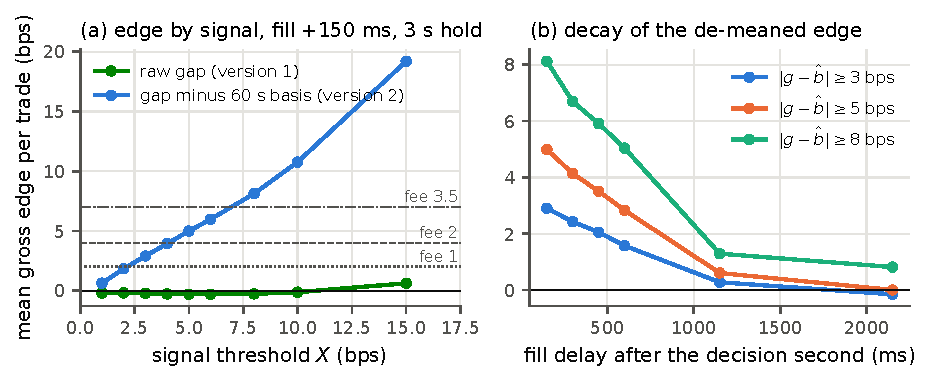
\includegraphics[width=\textwidth]{fig_train_signal.pdf}
\caption{Training days only (3--24 September). Every decision second with $|$signal$|\geq X$
enters 0.001\,BTC on HL in the signal direction at the recorded book 150\,ms later (depth VWAP
plus 0.1\bps{} slippage) and exits 3\,s later the same way. Gross edge includes spread and
slippage but not fees; a trade breaks even when gross edge equals twice the fee per side
(horizontal lines, labelled by fee). (a) Raw gap against the gap minus its 60\,s EMA basis.
(b) The de-meaned edge against the fill delay. From
\texttt{analysis/train\_signal\_analysis.json}.}
\label{fig:trainsignal}
\end{figure}

Figure~\ref{fig:trainsignal} shows the gross edge of each signal on the training days. A
trade triggered by the raw gap lost between 0.12 and 0.30\bps{} gross on average at every
threshold from 1 to 10\bps, before any fee; only the 3,098 signals at 15\bps{} or more over 22
days averaged a positive 0.63\bps, less than the two fees of a round trip even at 0.5\bps{}
per side. The
de-meaned gap earned 1.84\bps{} at a 2\bps{} threshold, 2.91\bps{} at 3\bps, 4.99\bps{} at
5\bps{} and 8.12\bps{} at 8\bps, and at a 3\bps{} threshold with a 1\bps{} fee per side its net
was positive on all 22 training days. The edge decays quickly after the signal: at the 3\bps{}
threshold it was 2.91\bps{} with the fill at 150\,ms, 2.05\bps{} at 450\,ms, 1.58\bps{} at
600\,ms and 0.28\bps{} at 1,150\,ms.

In the terms of Equation~\eqref{eq:decomp}, version~1's observation aliased the basis $b_t$
with the lead-lag term $u_t$. For an agent that sees only the raw gap on these training days,
entering with a 3\,s exit lost money at every measured threshold once fees are paid. One fixed
exit does not show that the best memoryless policy is always flat; a raw-gap rule that exits
when the gap closes made money at low fees on the later days (Table~\ref{tab:test450}). PPO
converged to near-abstention, which is consistent with the measurement. We attribute the
failure mainly to the observation; we did not train another optimiser on version~1's
observation. Version~2 also changed the decision epochs, made the fee an input and let the
agent learn the exit, so the test results below do not isolate the basis feature. Two pieces
of evidence still favour the basis explanation. On the test days a fixed-hold rule on the
de-meaned gap beat the version~1 raw-gap rule at 0.5 and 1\bps{} (Table~\ref{tab:test450}).
Also, on the six basis days, 18 to 23 September, between 21.9\% and 98.2\% of seconds had an absolute raw
gap of 7\bps{} or more, while only 0.011\% to 0.14\% had an absolute de-meaned gap that large,
the same range as on the other 16 training days (0.002\% to 0.19\%). The EMA removed the
offset that dominated version~1's training data.

% ------------------------------------------------------------------ 6
\section{Algorithms}\label{sec:algos}

All four learners used the same 22 training days, decision epochs, 20-feature observation,
fee sampling and validation selection rule. PPO was trained on the table built before the
amendment-3 fix, which differs from the rebuilt table used by the other three in 389 of about
14.3 million fill cells (Section~\ref{sec:limits}). Table~\ref{tab:algos} summarises what each
learner assumes and which question it answers. Appendix~\ref{app:hyper} lists every setting.

\begin{table}[!htbp]
\centering
\caption{The four learners. Time is wall-clock training time per seed on one CPU process,
from the saved run settings (450\,ms runs).}
\label{tab:algos}
\small
\begin{tabularx}{\textwidth}{@{}l>{\raggedright\arraybackslash}X>{\raggedright\arraybackslash}X r@{}}
\toprule
Learner & How it learns & Question it answers & Time/seed \\
\midrule
PPO & On-policy actor-critic; fresh rollouts from the fast replay; exploration by a stochastic
policy & Whether the proposal's main method learns entry and exit jointly once the state
is right & 1,591--1,613\,s \\
Double DQN & Off-policy value learning; replay buffer; random actions with a decaying
probability; Double-DQN target (Section~\ref{sec:ddqn}) & Whether replay of past transitions
and a value target do better than on-policy updates & 1,171--1,176\,s \\
FQI (stopping) + greedy entry & Batch regression on all counterfactual training paths; no
exploration & How far a method that exploits the exogenous dynamics gets with little
compute & 95--104\,s \\
Contextual bandit & One-step regression of the payoff of a fixed 3\,s trade & What the
learned exit adds & (in FQI run) \\
\bottomrule
\end{tabularx}
\end{table}

\subsection{PPO}
PPO~\cite{ppo} updates the policy by maximising the clipped surrogate objective
\begin{equation}
L^{\text{CLIP}}(\theta)=\hat{\E}_k\Bigl[\min\bigl(\rho_k(\theta)\hat A_k,\;
\operatorname{clip}(\rho_k(\theta),1-\epsilon,1+\epsilon)\hat A_k\bigr)\Bigr],\qquad
\rho_k(\theta)=\frac{\pi_\theta(a_k\mid o_k)}{\pi_{\theta_{\text{old}}}(a_k\mid o_k)},
\label{eq:ppo}
\end{equation}
with $\epsilon=0.2$ and advantages $\hat A_k$ from generalised advantage estimation~\cite{gae}
($\gamma=0.99$, $\lambda=0.95$), plus a value loss and an entropy bonus (coefficient 0.01, or
0.03 in half of the 150\,ms runs). The clip in Equation~\eqref{eq:ppo} removes any gain from
moving the probability ratio $\rho_k$ outside $[1-\epsilon,1+\epsilon]$, which keeps each
update close to the policy that collected the data. We used Stable-Baselines3~\cite{sb3} with
8 parallel environments and separate $64\times64$ tanh policy and value networks; each run
trained for 2,002,944 steps with checkpoints every 250,000 steps. Table~\ref{tab:hyper} in
Appendix~\ref{app:hyper} lists the remaining settings.

\subsection{Double DQN}\label{sec:ddqn}
DQN~\cite{dqn} learns $Q_\theta(o,a)$ from a replay buffer with a periodically copied target
network $\theta^-$. The standard target $r+\gamma\max_{a'}Q_{\theta^-}(o',a')$ takes a maximum
over noisy estimates and is biased upwards. In this task the bias reaches both actions of a
flat agent: $Q(\text{skip})$ through the maximum at the next flat epoch, and
$Q(\text{enter})$ through the maxima at the holding epochs that follow. Entering is followed
by a chain of holding epochs, each adding a maximum, so the overestimation may accumulate more
on the enter branch and favour entering. This is a bias in the targets. Noise in the estimate
of $Q(\text{enter})$ at the decision itself also leads to marginal entries, and the Double
target does not address that. Double DQN~\cite{ddqn} selects the next action with the online
network and evaluates it with the target network:
\begin{equation}
y=r+\gamma\,(1-\text{done})\;Q_{\theta^-}\!\Bigl(o',\,\arg\max_{a'}Q_\theta(o',a')\Bigr).
\label{eq:ddqn}
\end{equation}
We subclassed Stable-Baselines3's DQN to use this target with a Huber loss (squared error for
small errors, absolute error for large ones). Exploration was $\epsilon$-greedy: a random
action with probability $\epsilon$, decayed linearly from 1.0 to 0.02 over the first 20\% of
training. Seeds 7, 17 and 27 each ran for 1,000,000 steps with a hard target copy every 5,000
steps and checkpoints every 250,000 steps; Table~\ref{tab:hyper} lists the rest. Double DQN
is the value-based comparison the proposal promised.

\subsection{Fitted-Q iteration for the exit, with a greedy entry}\label{sec:fqi}
FQI~\cite{ernst} turns Bellman equations, here those of the stopping
problem~\eqref{eq:qexit}--\eqref{eq:qhold}, into a sequence of supervised regressions on a
fixed batch of transitions; with a neural network as the regressor it is neural fitted Q
iteration~\cite{nfq}. Exogeneity (Section~\ref{sec:exo}) supplies the batch without any
exploration. For every admissible training entry (a screened second where the entry would
fill), the recorded table gives the holding path and the exact payoff~\eqref{eq:payoff} of
exiting at each of the following seconds $h=1,\ldots,29$, together with the forced-exit payoff
$F_i$. Each of the 39,921 admissible entries was used twice with fees drawn from
$\mathcal{F}_{\text{train}}$, giving 79,842 paths. With features $\phi_{i,h}$ of path $i$ at
holding second $h$, exit payoff $X_{i,h}$ and last decision second $H_i$, each iteration $n$
computes
\begin{equation}
V^{(n)}_{i,h}=\max_{a\in\mathcal{A}_{i,h}}Q^{(n)}_{a}(\phi_{i,h}),
\qquad
y^{\text{hold}}_{i,h}=\begin{cases}V^{(n)}_{i,h+1} & h<H_i,\\ F_i & h=H_i,\end{cases}
\qquad y^{\text{exit}}_{i,h}=X_{i,h},
\label{eq:fqi}
\end{equation}
where $\mathcal{A}_{i,h}$ contains exit only if the book at that second can fill it, and fits
a two-headed network to these targets (the exit head only where an exit could fill). The
network is a $20\to64\to64\to2$ tanh perceptron trained with Adam at learning rate $10^{-3}$
and minibatches of 4,096. The loss is a Huber loss with a 2\bps{} threshold, so each head
estimates a robust central value of its targets (an M-estimate) rather than their mean. We
ran 15 iterations with one pass over the data each and kept the network between iterations.
The exit policy is to exit at the first second where $Q_{\text{exit}}\geq Q_{\text{hold}}$.

This is fitted value iteration of the stopping problem, in the spirit of regression-based
American option pricing, but it differs from the Longstaff--Schwartz method~\cite{lsm} in its
targets. Longstaff and Schwartz work backwards one date at a time and regress the realised
payoff of the current exercise rule, using fitted values only to decide when to exercise;
this avoids the upward bias of taking a maximum over fitted values. Our targets are maxima of
the fitted network at $h+1$, updated for all $h$ at once, as in the value-iteration variant of
Tsitsiklis and Van Roy~\cite{tvr}.

For the entry, the realised payoff $\Pi_i$ of each path under the learned exit was regressed on
the flat observation (fee included) for 8 epochs with the same Huber loss, and the agent enters
when the prediction is positive. This approximates the bandit rule of
Equation~\eqref{eq:entry}, enter when $\E[\Pi\mid x,f]>0$, with a robust central value in place
of the mean; it ignores the option of waiting for a larger gap and the cost of being busy.
Training took 95 to 104\,s per seed, about one sixteenth of PPO's time.

\subsection{Contextual-bandit ablation}
The bandit uses the same entry regression with every trade closed at the first fillable
second at least 3\,s after entry, the horizon of the training-day analysis. There is no
sequential decision after entry. Comparing it with FQI, which shares the entry method,
indicates what the learned exit adds; because the two entry regressions are fitted to
different payoffs, the two also enter on different seconds. Amendment~5 registered the
bandit's exit as the validation-tuned convergence rule at each fee; the implementation used the fixed 3\,s exit
instead. We report the bandit as implemented and treat this as a deviation from the protocol.

\subsection{Hand-written rules}
All rules ran in the same simulator with the same costs and windows. The version~1 raw-gap
rule enters at $|g_t|\geq X$ and exits when the directional raw gap is back to 0.5\bps. The
fixed-hold de-meaned rule uses the agent's screen, enters at $|\gt_t|\geq X$ and exits after
$H$ seconds. The convergence-exit de-meaned rule (added by amendment~2) enters at
$|\gt_t|\geq X$ and exits when the directional de-meaned gap falls to $E$\bps{} or after $H$
seconds. Each rule's $X$, $H$ and $E$ were tuned per fee on validation, which gives the rules
a per-fee advantage over the single fee-conditioned network. At every fee the
convergence-exit rule beat the fixed-hold rule on validation, so it is the primary
comparator; we call it the best rule (convergence exit), or the best rule for short.

\subsection{Algorithms we did not use}
Soft actor-critic~\cite{sac} and TD3~\cite{td3} were designed for continuous action spaces;
our action set has two elements, and a discrete variant of soft actor-critic would add an
entropy temperature to tune without a clear benefit. Model-based RL would have to learn
$P(x'\mid x)$ in the kernel~\eqref{eq:kernel}, a generative model of two order books, which is
harder than the control problem. Because of exogeneity every policy can be evaluated on the
same recorded paths without such a model. A learned model could still help a policy
generalise beyond those paths, but it would add model error. Offline methods such as
conservative Q-learning~\cite{cql} penalise actions that the logging policy rarely took, to
guard against distribution shift; counterfactual replay removes the policy-induced part of
that shift here. Recurrent policies would address partial
observability; the EMA basis covers the main hidden variable, and we kept feed-forward
networks to compare the algorithms on equal footing.

% ------------------------------------------------------------------ 7
\section{Protocol}\label{sec:protocol}
The protocol was written to a JSON file and registered at 02:15 UTC on 5 October 2026, before
any validation result of a version~2 checkpoint or baseline. Before that, the signal analysis
had used training days only, and a software check had replayed fixed rules on 60 validation
windows to compare the fast replay with the simulator; that check's P\&L was not used for any
choice. The protocol fixed the data splits, the fees, the candidate runs, the checkpoint
selection rule, the rule grids and three success criteria. Validation choices were frozen in
a selection file with its SHA-256 hash before the
simulator was run on test days, and the evaluation code refuses to run if the hash does not
match. Five amendments followed (Table~\ref{tab:amend}; full text in
Appendix~\ref{app:protocol}).

\begin{table}[!htbp]
\centering
\caption{Protocol amendments, with registration time (UTC, 5 October 2026) and what had been
seen at that point.}
\label{tab:amend}
\small
\begin{tabularx}{\textwidth}{@{}l l >{\raggedright\arraybackslash}X >{\raggedright\arraybackslash}X@{}}
\toprule
No. & Time & Change & Seen before registering \\
\midrule
1 & 02:30 & Add a 450\,ms group of three PPO runs trained, selected and tested at 450\,ms,
because received-book fills overstate the edge & No version~2 validation or test result \\
2 & 02:46 & Add the convergence-exit rule; widen its exit grid (2b) because the best level
sat on the grid edge & 150\,ms validation selection (PPO ahead of the fixed-hold rule by a
factor of two to four) \\
3 & 02:50 & Fix a floating-point error in the table's depth VWAP (0.002\% of fillable rows)
and a harsher-than-simulator forced-exit price in the fast replay; rebuild tables; re-run
selection, which made the same choices & 150\,ms validation selection; no test result \\
4 & 03:08 & 450\,ms group primary; per-fee rank-sum checkpoint selection; paired primary
endpoint; HL-clock stress; same-snapshot split; test sets labelled previously examined &
Partial 150\,ms test results at fees 0.5 and 1\bps{} (see text) \\
5 & 15:18 & Add Double DQN, FQI and the bandit ablation on the 450\,ms group & All PPO test
results of both groups; no training of the new algorithms \\
\bottomrule
\end{tabularx}
\end{table}

\paragraph{Selection.} The 150\,ms group chose one of 54 PPO checkpoints (six runs, nine
checkpoints each) by the sum of validation net P\&L over the four fees. Amendment~4 changed
the rule for the 450\,ms group to a per-fee rank sum, so that the 0.5\bps{} fee, where dollar
amounts are largest, does not decide alone: every checkpoint is ranked by validation net P\&L
at each fee, the ranks are summed, the lowest sum wins and ties go to fewer trades. Amendment~5
applied the same rule within each new algorithm. Rules were tuned per fee on validation net
P\&L.

\paragraph{Primary endpoint.} For each fee, the endpoint is the per-window difference
between PPO's net P\&L and the best rule's on identical test windows, summed over windows,
with a 90\% interval from a bootstrap that resamples whole UTC hours of windows (10,000
resamples), so that windows close in time are kept together. A comparison is inconclusive if
either policy has fewer than 100 test trades or the interval contains zero. A pooled
statistic across fees was registered as supporting evidence. Amendment~5 used
the same test for every algorithm against PPO and against the best rule. The original success
criteria (PPO above the version~1 raw-gap rule at every fee, and trading wherever its
validation P\&L was positive) were kept as secondary.

\paragraph{Previously examined test data.} The test days of 29 September to 2 October were
opened by version~1's attempt~1, which ran its threshold rule on them at fees from 0.5 to
3.5\bps. The day of 3 October was opened by version~1's expected-value diagnostic (attempt~3
in the protocol), which made one trade. Neither set was used directly in version~2's design,
but version~1's summary statistics and rule results on these days were known to the team, so
both are previously examined, not confirmatory. Amendment~4 records that partial 150\,ms test
results at 0.5 and 1\bps{} had been seen when it made the 450\,ms group primary; it does not
record which policies were looked at. The simulator files for those two fees, written before
the amendment, show PPO level with the convergence rule (\usd{107.82} against \usd{108.29} and
\usd{66.07} against \usd{65.69}; Table~\ref{tab:lat150}). Days from 4 October onward would be
confirmatory; they were not exported in this session. A script
(\texttt{latency\_arb/v2/confirm.py}) evaluates the frozen PPO and rule choices of both
latency groups on newly prepared days without any retraining or reselection; it does not yet
cover the amendment-5 algorithms.

% ------------------------------------------------------------------ 8
\section{Results}\label{sec:results}

\subsection{Validation selection}
Table~\ref{tab:val450} gives each frozen choice's validation result at 450\,ms and
Figure~\ref{fig:valcand} shows every candidate (Appendix~\ref{app:candidates} lists the
Double DQN, FQI and bandit candidates). The rank sum chose PPO seed~27 at 750,000
steps; the sum of dollars would have chosen the same run at 2,000,000 steps (\usd{63.38}
against \usd{62.29} summed over fees). For Double DQN it chose seed~27 at 1,000,000 steps,
for FQI seed~17 and for the bandit seed~27. On validation PPO led at 0.5 and 1\bps, Double
DQN and FQI were close at 0.5\bps{} (about \usd{29} each) with Double DQN ahead at 1\bps, and
the bandit was far behind, the same order as on the test days. PPO's 27 checkpoints fell in a
narrow band at 0.5\bps{} (\usd{37.57} to \usd{41.65}, with the chosen checkpoint at the top) and
spread more widely at 2 and 3.5\bps, where trade counts are small.

\begin{table}[!htbp]
\centering
\caption{Validation (25--28 September, 1,117 windows), fill at 450\,ms, frozen choices only.
Net P\&L in US dollars for 0.001\,BTC per trade, with the number of trades. Validation numbers
come from the fast replay (Section~\ref{sec:env}).}
\label{tab:val450}
\small
\setlength{\tabcolsep}{4.5pt}
\begin{tabular}{@{}lrrrrrrrr@{}}
\toprule
 & \multicolumn{2}{c}{0.5\bps} & \multicolumn{2}{c}{1\bps} & \multicolumn{2}{c}{2\bps} & \multicolumn{2}{c}{3.5\bps} \\
\cmidrule(lr){2-3}\cmidrule(lr){4-5}\cmidrule(lr){6-7}\cmidrule(l){8-9}
Policy & Net & Trades & Net & Trades & Net & Trades & Net & Trades \\
\midrule
\tabinput{generated/tab_val450.tex}
\bottomrule
\end{tabular}
\end{table}

\begin{figure}[!htbp]
\centering
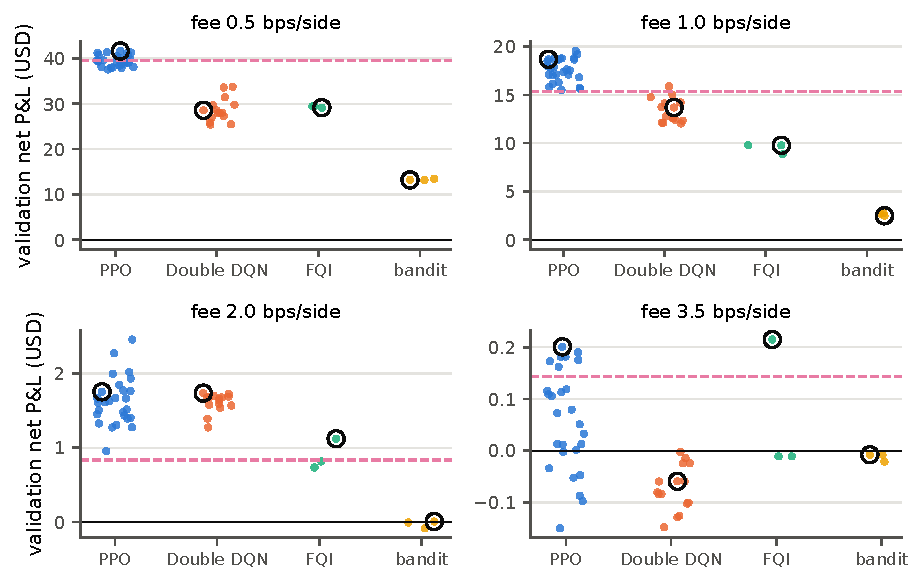
\includegraphics[width=\textwidth]{fig_validation_candidates.pdf}
\caption{Validation net P\&L at 450\,ms of every candidate: 27 PPO checkpoints, 15 Double DQN
checkpoints (five per seed), and three seeds each of FQI and the bandit. Circles mark the
frozen choices; the dashed line is the best rule tuned at that fee.}
\label{fig:valcand}
\end{figure}

\subsection{Primary test: \texorpdfstring{450\,ms}{450 ms}, test A}
Table~\ref{tab:test450} and Figure~\ref{fig:algos} give the single test run of every frozen
choice in the unchanged simulator. PPO's net P\&L was positive at every fee, from \usd{76.91}
over 5,056 trades at 0.5\bps{} to \usd{0.05} over 45 trades at 3.5\bps. A bootstrap that
resamples the four test days gives 90\% intervals of \usd{67.26} to \usd{86.56} at 0.5\bps,
\usd{32.00} to \usd{43.75} at 1\bps, \usd{1.11} to \usd{3.31} at 2\bps{} and $-$\usd{0.09} to
\usd{0.21} at 3.5\bps, so the 3.5\bps{} result cannot be told apart from zero. PPO's net P\&L
was positive on all four test days at 0.5 and 1\bps, on three of four at 2\bps{} and on two of
four at 3.5\bps. Double DQN made
\usd{54.61}, \usd{25.29}, \usd{3.17} and \usd{0.02}; FQI \usd{55.37}, \usd{20.33}, \usd{0.80}
and $-$\usd{0.06}; the bandit \usd{25.51}, \usd{4.49}, \usd{0.76} and \usd{0.05}. The best rule
made \usd{76.77}, \usd{34.80}, \usd{1.94} and \usd{0.05}, and the version~1 raw-gap rule
\usd{23.92}, \usd{3.78}, \usd{0.67} and \usd{0.00}. The largest drawdown (peak-to-trough fall
in cumulative P\&L) of any learner at 0.5 or 1\bps{} was \usd{0.60} (FQI at 1\bps). The
amounts are small because each trade is
0.001\,BTC, about \usd{84}; at 0.5\bps{} PPO's \usd{76.91} is 1.8\bps{} of notional per trade.

\begin{table}[!htbp]
\centering
\caption{Primary test (test~A: 29 September to 2 October, 1,140 windows), fill at 450\,ms,
unchanged simulator. Net P\&L in US dollars and number of trades. Learners above the line,
rules below.}
\label{tab:test450}
\small
\setlength{\tabcolsep}{4.5pt}
\begin{tabular}{@{}lrrrrrrrr@{}}
\toprule
 & \multicolumn{2}{c}{0.5\bps} & \multicolumn{2}{c}{1\bps} & \multicolumn{2}{c}{2\bps} & \multicolumn{2}{c}{3.5\bps} \\
\cmidrule(lr){2-3}\cmidrule(lr){4-5}\cmidrule(lr){6-7}\cmidrule(l){8-9}
Policy & Net & Trades & Net & Trades & Net & Trades & Net & Trades \\
\midrule
\tabinput{generated/tab_test450.tex}
\bottomrule
\end{tabular}
\end{table}

\begin{figure}[!htbp]
\centering
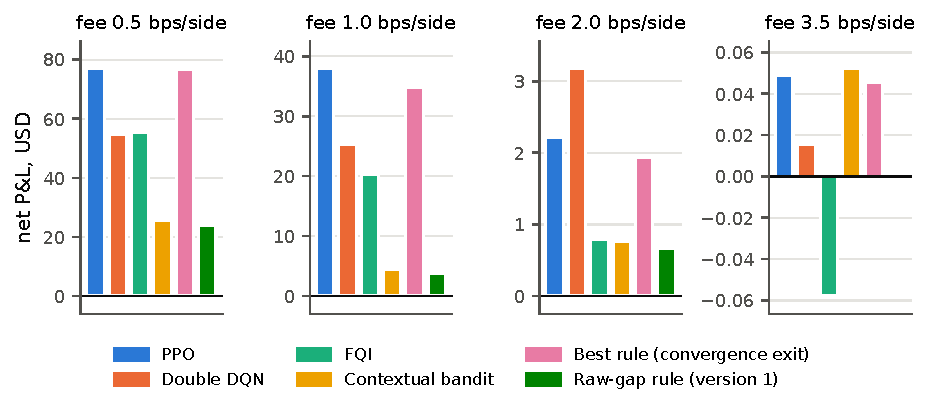
\includegraphics[width=\textwidth]{fig_algos_by_fee.pdf}
\caption{Primary test, net P\&L by fee (each panel has its own scale). Values are in
Table~\ref{tab:test450}.}
\label{fig:algos}
\end{figure}

\subsection{Paired comparisons}
Table~\ref{tab:paired} and Figure~\ref{fig:paired} give the registered paired statistics.
Against the best rule, PPO was level at 0.5\bps{} (\usd{0.14}, interval $-$\usd{1.92} to
\usd{1.99}; ahead on 1 of 4 days) and conclusively ahead at 1\bps{} (\usd{3.12}, interval
\usd{0.80} to \usd{5.34}; ahead on all 4 days and in 67 of 96 hours). At 2 and 3.5\bps{} the
intervals contained zero. The pooled statistic sums the per-window differences over all four
fees after dividing each by the rule's validation per-window standard deviation at that fee,
so one unit is one such standard deviation. It was 83.0 with an interval from $-$33.0 to
200.8, so it was also inconclusive.

PPO was conclusively ahead of Double DQN, FQI and the bandit at 0.5 and 1\bps, by \usd{12.62}
to \usd{51.40}, and ahead on every test day in each of these six comparisons. At 2\bps{} Double
DQN was conclusively ahead of PPO by \usd{0.96} (interval \usd{0.12} to \usd{1.87}) and also
ahead of the best rule by \usd{1.23} (interval \usd{0.48} to \usd{2.06}), with 240 trades
against PPO's 628 and the rule's 210. At 3.5\bps{} no learner made 100 trades and every
comparison was inconclusive. Against the version~1 raw-gap rule PPO was ahead at 0.5 and
1\bps; at 2 and 3.5\bps{} that rule made 15 and 0 trades, too few for a verdict.

\begin{table}[!htbp]
\centering
\caption{Paired comparisons on the primary test (test~A, 1,140 windows, 450\,ms). Difference is PPO
minus the other policy, summed over windows, in US dollars; the interval is the 90\% hour-block
bootstrap interval. ``Days'' counts days on which PPO was ahead. A verdict needs at least 100
trades for both policies and an interval that excludes zero. PPO's trades were 5,056, 3,813,
628 and 45.}
\label{tab:paired}
\small
\setlength{\tabcolsep}{5pt}
\begin{tabular}{@{}llrrrrl@{}}
\toprule
Fee & Other policy & Its trades & Difference & 90\% interval & Days & Verdict \\
\midrule
\tabinput{generated/tab_paired450.tex}
\bottomrule
\end{tabular}
\end{table}

\begin{figure}[!htbp]
\centering
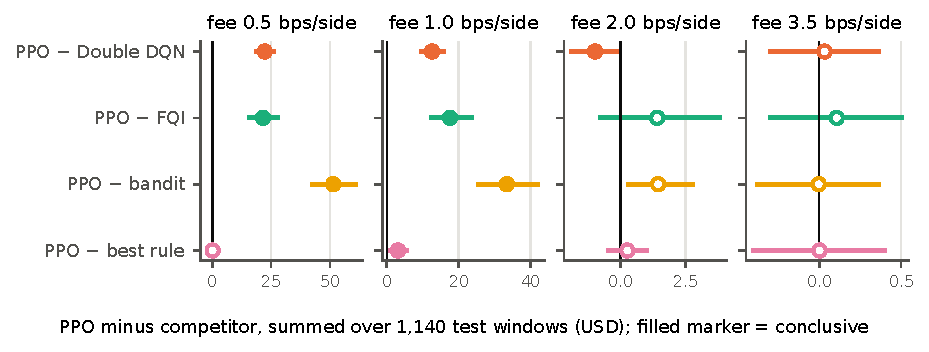
\includegraphics[width=\textwidth]{fig_paired.pdf}
\caption{PPO minus each competitor on the primary test, with 90\% hour-block bootstrap
intervals. Positive values favour PPO. Hollow markers are inconclusive by the registered rule
(interval contains zero, or fewer than 100 trades); the bandit at 2\bps{} has an interval that
excludes zero but only 66 trades.}
\label{fig:paired}
\end{figure}

\subsection{Fee-dependent selectivity}
One PPO network served all four fees. Its trade count fell from 5,056 at 0.5\bps{} to 3,813,
628 and 45 as the fee rose (Figure~\ref{fig:select}). The best rule, tuned per fee, used the
same setting at 0.5 and 1\bps{} (enter at 2\bps, exit at $-1$\bps{} or after 30\,s) and made
4,972 trades at both fees; it became selective only at 2\bps, with 210 trades.
Table~\ref{tab:pertrade} breaks the trades down. At 1\bps{} PPO made 1,159 fewer trades than
the rule, earned 1.18\bps{} net per trade against the rule's 0.83, and held 11.7\,s on average
against 13.7\,s. PPO's advantage at 1\bps{} came from these fewer trades at a higher net edge
per trade. At 2\bps{} the order
reversed: PPO made three times as many trades as the rule and 2.6 times as many as Double DQN,
at 0.41\bps{} net per trade against 1.09 and 1.56. Double DQN entered less often than PPO at
every fee; that cost it at 0.5 and 1\bps, where many marginal trades were still profitable,
and paid off at 2\bps.

\begin{figure}[!htbp]
\centering
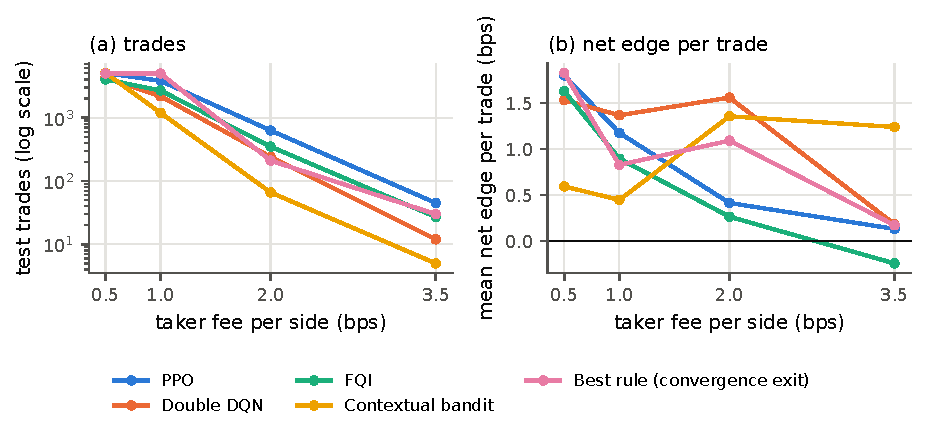
\includegraphics[width=\textwidth]{fig_selectivity.pdf}
\caption{Primary test. (a) Trades by fee, log scale. (b) Mean net P\&L per trade in bps of
entry notional. At 3.5\bps{} the means rest on 5 to 45 trades.}
\label{fig:select}
\end{figure}

\begin{table}[!htbp]
\centering
\caption{Per-trade economics on the primary test. Gross and net are mean bps of entry
notional per trade; gross includes spread and slippage but not fees. ``Policy exits'' are exits
the policy chose; ``30\,s exits'' hit the holding limit (the rest closed at the window end).
The bandit chooses no exit: every trade closes after its fixed 3\,s hold.}
\label{tab:pertrade}
\small
\setlength{\tabcolsep}{3.5pt}
\begin{tabular}{@{}llrrrrrrr@{}}
\toprule
Fee & Policy & Trades & Gross & Net & Win \% & Hold (s) & Policy exit \% & 30\,s exit \% \\
\midrule
\tabinput{generated/tab_pertrade450.tex}
\bottomrule
\end{tabular}
\end{table}

\subsection{The \texorpdfstring{150\,ms}{150 ms} group as an optimistic sensitivity}
The original protocol's 150\,ms group trained six PPO runs and selected seed~27 (entropy
0.01) at its final checkpoint. With fills at 150\,ms everything earned more
(Table~\ref{tab:lat150}): PPO made \usd{107.82} at 0.5\bps{} and \usd{13.51} at 2\bps. Against
the best rule, PPO was level at 0.5 and 1\bps{} and conclusively ahead at 2\bps{}
(\usd{4.45}, interval \usd{2.33} to \usd{6.92}); at 3.5\bps{} the rule made only 33 trades.
Amendment~4, written after an independent review and following amendment~1's finding that
received-book fills at 150\,ms overstate the edge, made the 450\,ms group primary and this group
an optimistic sensitivity analysis. The same-snapshot split that amendment~4 registered later
showed that 71\% of this group's test entries at 0.5\bps{} (3,797 of 5,340) filled at the HL
snapshot the decision had already seen. The two groups agree that PPO and the best rule are
close at 0.5\bps{} and disagree on whether PPO's advantage appears at 1 or at 2\bps.

\begin{table}[!htbp]
\centering
\caption{The 150\,ms group. Top: validation (selection files) and both test sets, net P\&L in
US dollars and trades. Bottom: paired comparison of PPO with the best rule on test~A (90\%
hour-block bootstrap interval; same verdict rule as Table~\ref{tab:paired}).}
\label{tab:lat150}
\small
\setlength{\tabcolsep}{4.5pt}
\begin{tabular}{@{}lrrrrrrrr@{}}
\toprule
 & \multicolumn{2}{c}{0.5\bps} & \multicolumn{2}{c}{1\bps} & \multicolumn{2}{c}{2\bps} & \multicolumn{2}{c}{3.5\bps} \\
\cmidrule(lr){2-3}\cmidrule(lr){4-5}\cmidrule(lr){6-7}\cmidrule(l){8-9}
Policy & Net & Trades & Net & Trades & Net & Trades & Net & Trades \\
\midrule
\tabinput{generated/tab_lat150.tex}
\bottomrule
\end{tabular}

\vspace{8pt}
\begin{tabular}{@{}lrrrrl@{}}
\toprule
Fee & PPO (trades) & Best rule (trades) & Difference & 90\% interval & Verdict \\
\midrule
\tabinput{generated/tab_paired150.tex}
\bottomrule
\end{tabular}
\end{table}

\subsection{Test B: 3 October}
On 3 October (285 windows) every policy made under 125 trades at each fee and all amounts were
below one dollar (Table~\ref{tab:testB}). PPO made \usd{0.69} at 0.5\bps{} and lost \usd{0.03}
and \usd{0.16} at 1 and 2\bps; the best rule lost \usd{0.45} at 1\bps. Most paired comparisons
were inconclusive because of the trade-count rule. Three were not, all at 0.5\bps: PPO was
ahead of FQI (\usd{0.17}, interval \usd{0.02} to \usd{0.34}) and of the bandit (\usd{0.44},
interval \usd{0.24} to \usd{0.69}), and the best rule was ahead of the bandit (\usd{0.33},
interval \usd{0.19} to \usd{0.48}). The day had the smallest gaps of the whole dataset (median
absolute gap 0.61\bps) and says little either way.

\begin{table}[!htbp]
\centering
\caption{Test~B (3 October, 285 windows), fill at 450\,ms, unchanged simulator. Net P\&L in
US dollars and number of trades.}
\label{tab:testB}
\small
\setlength{\tabcolsep}{4.5pt}
\begin{tabular}{@{}lrrrrrrrr@{}}
\toprule
 & \multicolumn{2}{c}{0.5\bps} & \multicolumn{2}{c}{1\bps} & \multicolumn{2}{c}{2\bps} & \multicolumn{2}{c}{3.5\bps} \\
\cmidrule(lr){2-3}\cmidrule(lr){4-5}\cmidrule(lr){6-7}\cmidrule(l){8-9}
Policy & Net & Trades & Net & Trades & Net & Trades & Net & Trades \\
\midrule
\tabinput{generated/tab_testB450.tex}
\bottomrule
\end{tabular}
\end{table}

\subsection{Learning curves}
Figure~\ref{fig:learning} shows training on the 450\,ms group. In its first rollout (4,096
steps, before smoothing) PPO took about half of the screened entries and lost 8.6 to 9.7\bps{}
of notional per window; the smoothed curves in the figure start at less extreme values
because each point averages up to ten log points. Its entry share
then fell to between 2\% and 5\% (smoothed) after 61,000 to 78,000 steps, the same move toward
abstention that version~1 made, but here it recovered: training reward per window turned
positive after 61,000 to 82,000 steps, and after one million steps the entry share settled at
21\% to 24\% and the reward at 2.0 to 2.1\bps{} per window for all three seeds. Unlike
version~1, the runs logged PPO's optimisation statistics (Appendix~\ref{app:curves}): after
one million steps the approximate Kullback--Leibler (KL) divergence between successive
policies averaged about 0.001 per update and the value
function explained about 56\% of the return variance. Double DQN's entry share fell from about
one half to 17\% to 18\% as $\epsilon$ decayed, its reward turned positive after 180,000 to
190,000 steps and settled at 1.4 to 1.5\bps{} per window, still with 2\% random actions. The
three seeds of each algorithm followed nearly the same path. Training rewards are not
comparable across the two algorithms, because PPO samples from a stochastic policy and DQN
acts $\epsilon$-greedily.

\begin{figure}[!htbp]
\centering
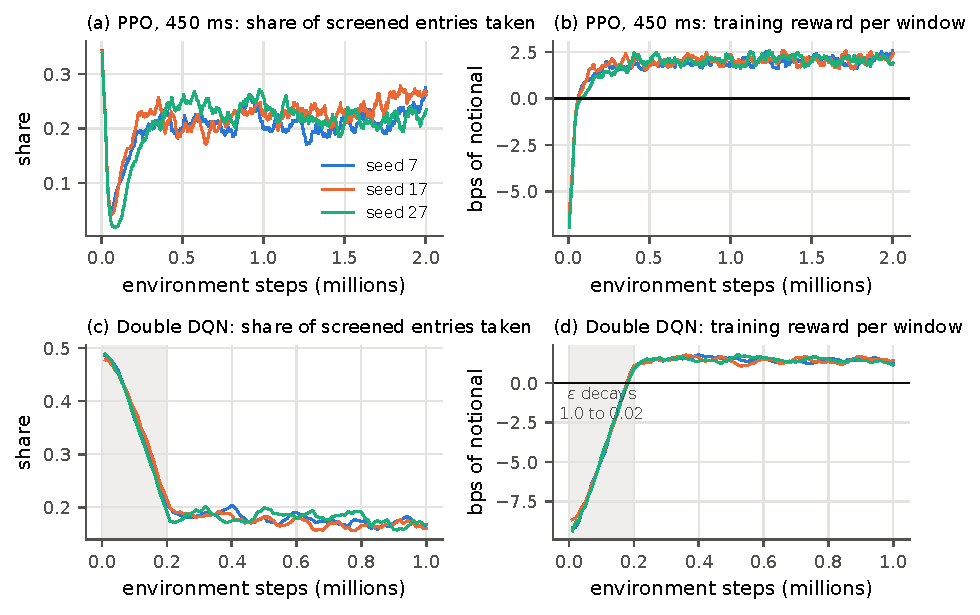
\includegraphics[width=\textwidth]{fig_learning.pdf}
\caption{Training curves, 450\,ms fills, three seeds each, smoothed over ten log points (five
for DQN). Entry share is the fraction of screened flat decisions on which the agent entered.
The shaded band in (c) and (d) is the $\epsilon$-decay phase. The 150\,ms PPO curves are in
Appendix~\ref{app:curves}.}
\label{fig:learning}
\end{figure}

\begin{figure}[!htbp]
\centering
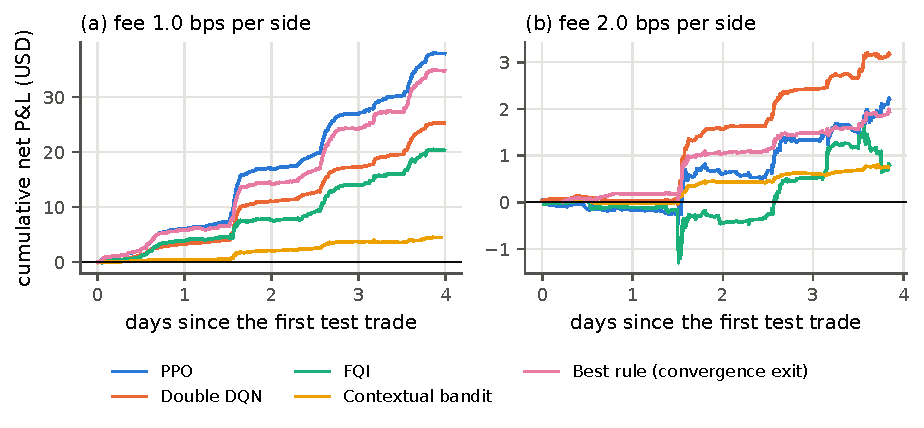
\includegraphics[width=\textwidth]{fig_cumulative.pdf}
\caption{Cumulative net P\&L over the primary test, trades ordered by exit time. Per-day
values are in Appendix~\ref{app:perday}.}
\label{fig:cum}
\end{figure}

Figure~\ref{fig:cum} shows how the test P\&L accumulated. At 1\bps{} PPO and the best rule
rose in steps during the same busy periods, and PPO pulled ahead at the larger steps. At
2\bps{} most of the differences arose on 30 September, when Double DQN made \usd{1.53} and FQI
lost \usd{0.35} (Appendix~\ref{app:perday}).

% ------------------------------------------------------------------ 9
\section{Stress tests}\label{sec:stress}
The frozen 450\,ms choices were replayed under harsher assumptions without reselection
(Table~\ref{tab:stress}, Figure~\ref{fig:stress}; full grid in Appendix~\ref{app:stress}).

\paragraph{Latency.} Every additional 150\,ms of fill delay cost PPO about \usd{15} to \usd{18} at
0.5\bps. At 600\,ms PPO still made \usd{58.96} and \usd{23.88} at 0.5 and 1\bps, but lost
\usd{0.61} at 2\bps, where the best rule kept \usd{0.91}.

\paragraph{Spread.} With every book level's distance from the mid scaled by 1.5, PPO made
\usd{71.11}, \usd{33.42}, \usd{1.21} and $-$\usd{0.05}.

\paragraph{Fee 4.5\bps{} (extrapolation).} PPO was given a fee of 4.5\bps, outside its training
range, and the rules kept their 3.5\bps{} settings. PPO cut its trades to 13 and lost
\usd{0.10}; the best rule made 30 trades and lost \usd{0.46}; the raw-gap rule did not trade.

\paragraph{HL-clock fills.} This is the strictest convention we could compute
(Table~\ref{tab:hlclock}); at 450\,ms it combines the order delay with HL's publication lag
(Section~\ref{sec:filltiming}). At 0.5\bps{} PPO made \usd{27.05}, the best rule \usd{26.11},
FQI \usd{17.86}, Double DQN \usd{11.58} and the raw-gap rule \usd{4.23}, while the bandit lost
\usd{13.69} and the fixed-hold rule \usd{4.09}. At 1\bps{} and above
every policy that traded lost money, including PPO ($-$\usd{4.62}, $-$\usd{10.07} and
$-$\usd{2.21}). On 3 October every policy that traded lost money at every fee under this
convention, except the raw-gap rule's three trades at 1\bps{} (\usd{0.01}).

\paragraph{Same-snapshot share.} Table~\ref{tab:samesnap} splits PPO's received-book results by
whether the entry filled at the same HL snapshot the decision saw. At 450\,ms 19\% of entries
did, and they produced \usd{19.27} of the \usd{76.91} at 0.5\bps. At 150\,ms the share was
71\%, at 600\,ms 1\%. Under HL-clock fills it was 1\% (45 of 5,049 entries).

\begin{table}[!htbp]
\centering
\caption{Stress tests on test~A for the frozen 450\,ms choices: PPO / best rule, net P\&L in US
dollars (fast replay; its 450\,ms column equals the simulator's). Trade counts are in
Appendix~\ref{app:stress}.}
\label{tab:stress}
\small
\setlength{\tabcolsep}{4pt}
\begin{tabular}{@{}lrrrrrr@{}}
\toprule
Fee & 150\,ms & 300\,ms & 450\,ms & 600\,ms & Spread $\times1.5$ & HL clock \\
\midrule
\tabinput{generated/tab_stress450.tex}
\bottomrule
\end{tabular}
\end{table}

\begin{figure}[!htbp]
\centering
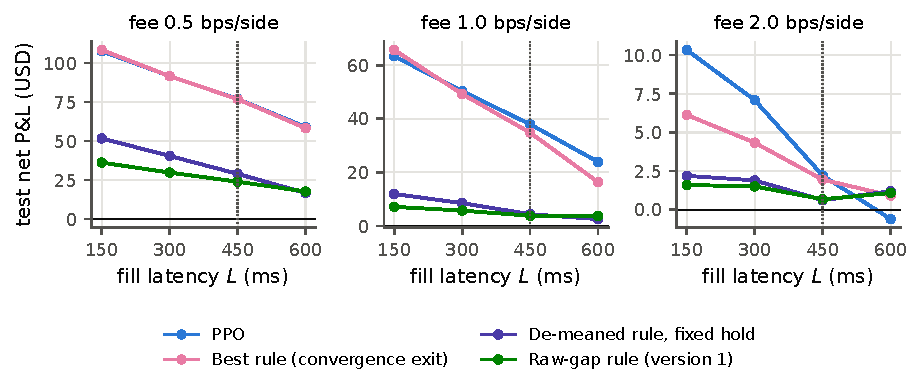
\includegraphics[width=\textwidth]{fig_stress_latency.pdf}
\caption{Test net P\&L of the frozen 450\,ms PPO choice and the rules when the same decisions
are filled 150 to 600\,ms after the decision (received-book convention). The dotted line marks
the primary latency.}
\label{fig:stress}
\end{figure}

\begin{table}[!htbp]
\centering
\caption{HL-clock fills at 450\,ms on test~A: fills priced from the last HL book whose exchange
timestamp is at or before $t+450$\,ms. Net P\&L in US dollars and trades.}
\label{tab:hlclock}
\small
\setlength{\tabcolsep}{3.2pt}
\begin{tabular}{@{}lrrrrrrrrrrrr@{}}
\toprule
 & \multicolumn{2}{c}{PPO} & \multicolumn{2}{c}{Double DQN} & \multicolumn{2}{c}{FQI} &
\multicolumn{2}{c}{Bandit} & \multicolumn{2}{c}{Best rule} & \multicolumn{2}{c}{Raw-gap rule} \\
\cmidrule(lr){2-3}\cmidrule(lr){4-5}\cmidrule(lr){6-7}\cmidrule(lr){8-9}\cmidrule(lr){10-11}\cmidrule(l){12-13}
Fee & Net & Tr. & Net & Tr. & Net & Tr. & Net & Tr. & Net & Tr. & Net & Tr. \\
\midrule
\tabinput{generated/tab_hlclock450.tex}
\bottomrule
\end{tabular}
\end{table}

\begin{table}[!htbp]
\centering
\caption{PPO entries (450\,ms choice, test~A) that filled at the same HL snapshot the decision
saw, by fill latency, with the net P\&L those trades produced out of the total
(received-book convention).}
\label{tab:samesnap}
\small
\begin{tabular}{@{}rllll@{}}
\toprule
 & \multicolumn{2}{c}{Fee 0.5\bps} & \multicolumn{2}{c}{Fee 1\bps} \\
\cmidrule(lr){2-3}\cmidrule(l){4-5}
Latency (ms) & Same-snapshot entries & Their net (\$) & Same-snapshot entries & Their net (\$) \\
\midrule
\tabinput{generated/tab_samesnap.tex}
\bottomrule
\end{tabular}
\end{table}

% ------------------------------------------------------------------ 10
\section{Discussion: what the algorithms learned}\label{sec:discussion}

\subsection{A path-dependent exit was worth more than a fixed hold}\label{sec:exitvalue}
The bandit and FQI share the entry method and differ in the exit. With its fixed 3\,s exit
the bandit made \usd{25.51} and \usd{4.49} at 0.5 and 1\bps, against FQI's \usd{55.37} and
\usd{20.33}. Their entry regressions were fitted to different payoffs, so they also entered on
different seconds (1,193 against 2,685 trades at 1\bps), and this comparison does not separate
the exit from the entry. On the 79,842 training paths, the same paths the exit network was
fitted to, FQI's learned exit raised the mean payoff over all admissible entries from $-2.67$
to $-2.69$\bps{} under the 3\,s exit to $-1.63$ to $-1.68$\bps{} (ranges over seeds), about
1\bps{} per trade before any entry selection; this is an in-sample figure. Among the rules,
both de-meaned rules entered at the same 2\bps{} threshold at 0.5\bps{} and made similar
numbers of trades (4,972 and 4,886). There the convergence exit made \usd{76.77} against the
fixed hold's \usd{28.95}, 2.7 times as much. At 1\bps{} the tuned rules differ in threshold as
well as exit (2 against 4\bps; 4,972 against 508 trades), so their ratio (\usd{34.80} against
\usd{4.34}) does not measure the exit alone. A path-dependent exit, whether learned or
hand-written, was worth much more than a fixed hold; we did not isolate the contribution of
learning the exit.

\subsection{PPO against a hand-written convergence rule}
At 0.5\bps{} PPO and the best rule were indistinguishable: similar trade counts (5,056 and
4,972), similar net edge per trade (1.80 and 1.83\bps) and a paired difference of 14 cents
over four days. At that fee a three-parameter rule tuned on four validation days captured
what PPO learned from 22 training days. PPO's advantage appeared at 1\bps, where it entered
more selectively than a rule whose validation tuning kept the 0.5\bps{} setting: the
fee-conditioned network cut its trades by 25\% between 0.5 and 1\bps, while the rule's grid
search returned the same setting at both fees. The difference is \usd{3.12} over four days.

\subsection{Double DQN's selectivity at \texorpdfstring{2\bps}{2 bps}}
Double DQN entered less often than PPO at every fee. At 0.5, 1 and 3.5\bps{} it also held for
shorter times (4.8\,s against 10.8\,s, 7.5 against 11.7\,s and 10.2 against 12.3\,s); at
2\bps{} the holds were about equal (10.9 against 10.8\,s). Its win at 2\bps, where most screened
entries no longer cover the fee, came from fewer entries with a higher edge: 240 trades at
5.56\bps{} gross against PPO's 628 at 4.41\bps. Low-fee windows carry most of PPO's training
reward and dominate its gradient, which may explain its extra trades at 2\bps. The Double
target may explain DQN's caution, because it reduces the upward bias in the targets
(Section~\ref{sec:ddqn}). We did not run plain DQN, so we cannot attribute the difference to
the target. Only the selected Double DQN, FQI and bandit policies were run on the test days,
so the spread between seeds and checkpoints on test is known for PPO only
(Appendix~\ref{app:runs}); we cannot say whether the 2\bps{} result holds for other
checkpoints of either learner.

\subsection{What FQI's greedy entry and fitted exit give up}
FQI trained in under two minutes per seed and reached 72\% of PPO's test P\&L at 0.5\bps{} and
54\% at 1\bps. Two simplifications cost it. First, its entry rule enters whenever the
predicted payoff is positive and so ignores the option value of waiting and the cost of being
busy (Equation~\eqref{eq:entry}). Second, its exit held too long: 21.5\,s on average at
1\bps{} against PPO's 11.7\,s, with 24\% of trades reaching the 30\,s limit against 10\%. On
the training paths the fitted value at the first holding second averaged 0.83 to 0.98\bps{}
(computed from the network before its last fit), while the same paths under the learned exit
realised $-1.63$ to $-1.68$\bps. Four causes are consistent with this gap of about 2.5\bps{}
and with the long holds. The targets in Equation~\eqref{eq:fqi} take a maximum over fitted
values, which is biased upwards and inflates the value of holding; Longstaff--Schwartz targets
avoid this bias and the Double DQN target reduces it. The stopping problem leaves out the value of being
flat after an exit (Section~\ref{sec:exo}), which lowers the value of exiting. The Huber loss
fits a robust central value, which differs from the mean when payoffs are skewed. And 15
iterations of one pass each are fewer than the 29 backward steps that exact backward
induction over the holding horizon would need. We did not run the experiments that would
separate these causes.

\subsection{When supervised or bandit methods would be enough}
If the exit is fixed, the entry problem is close to a contextual bandit
(Section~\ref{sec:exo}), and a regression on counterfactual payoffs is the natural method.
The bandit ablation did poorly with its fixed 3\,s exit. A bandit with the convergence exit,
the version the protocol registered, was not run and might close much of the gap. The
evidence here suggests that a path-dependent exit pays (Section~\ref{sec:exitvalue}) and that a learned,
fee-conditioned policy helps when one policy must serve many cost levels (the 1\bps{}
result). For a single known fee, a tuned rule with a convergence exit matched PPO.

% ------------------------------------------------------------------ 11
\section{Would faster order-book feeds help?}\label{sec:faster}
If the HL-clock convention is right, the estimates below say yes, mainly through two
changes: deciding on Binance events instead of whole seconds, and a faster view of HL's book.
A faster Binance stream alone adds little. The numbers come from the sub-second analysis on
six training days (4, 8, 12, 15, 19 and 23 September) with a fixed 3\,s exit, so they estimate
what a faster feed could add to a fixed 3\,s rule; no learned agent was tested on sub-second
data.

\begin{figure}[!htbp]
\centering
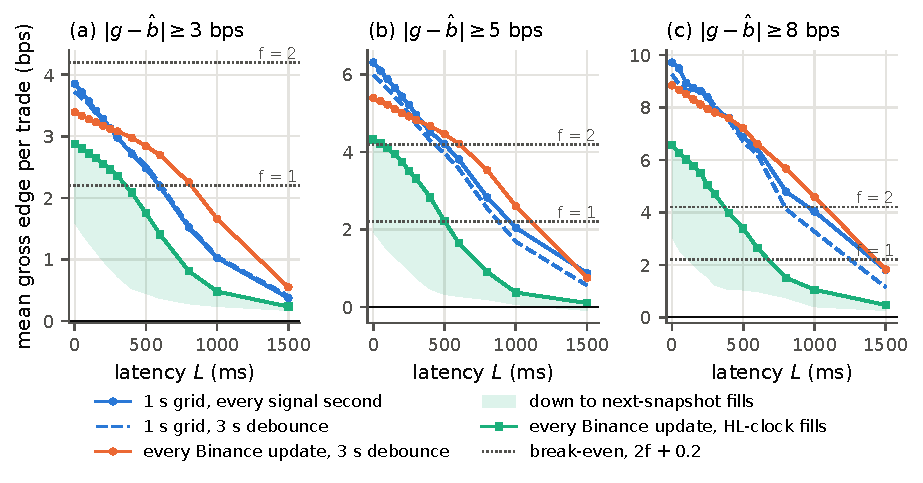
\includegraphics[width=\textwidth]{fig_edge_latency.pdf}
\caption{Sub-second analysis on six training days: mean gross edge of a 3\,s round trip on HL
against execution latency, for de-meaned gaps of at least 3, 5 and 8\bps. Blue: one-second
decision grid. Orange: decisions at every Binance update. Green: decisions at every Binance
update with HL-clock fills; the shaded band extends down to next-snapshot fills. Solid blue
counts every signal second; dashed blue and the event-driven curves apply a 3\,s debounce (no
new signal is counted within 3\,s of the previous one). Received-book fills except where
marked. In this analysis gross edge excludes slippage, so the dotted break-even lines sit at
twice the fee plus 0.2\bps, for fees $f$ of 1 and 2\bps{} per side. Redrawn from
\texttt{analysis/subsecond\_edge.json}.}
\label{fig:edgelat}
\end{figure}

\paragraph{The edge is perishable.} At a 3\bps{} threshold the gross edge fell from 3.86\bps{} with
an immediate fill to 3.41 at 150\,ms, 2.98 at 300\,ms, 2.48 at 500\,ms and 1.02 at 1,000\,ms,
about 0.28\bps{} per 100\,ms of delay (Figure~\ref{fig:edgelat}).

\paragraph{The one-second grid misses and delays dislocations.} A dislocation, the time the
de-meaned gap stays beyond the threshold, lasted 618, 510 and 306\,ms at the median for
thresholds of 3, 5 and 8\bps. The grid never saw 28.5\%, 36.0\% and 47.6\% of these onsets
within 10\,s, and when it did see one it added 452\,ms of delay at the median. Under
received-book fills this delay looks almost free (0.06\bps{} per trade), because the received
book is itself stale. Under HL-clock fills, waiting for the grid cost 1.0 to 1.9\bps{} per
trade. Daily net P\&L summed over trades at 1\bps{} per side and a 3\bps{} threshold, with
HL-clock fills, was $-78$\bps{} for the grid, $+330$\bps{} for event-driven decisions and
$+538$\bps{} for event-driven decisions with an emulated zero-delay view of HL's book.

\paragraph{Event-driven decisions change the epochs, the discount and the state's clock.} In
the model of Section~\ref{sec:smdp}, deciding on every Binance update replaces the
whole-second epochs with Binance event times: the screen~\eqref{eq:screen} is evaluated at each
update, sojourn times become random intervals of about 100\,ms for the depth stream, and the
per-epoch discount in the objective~\eqref{eq:objective} should become $\gamma^{\tau_k}$. The
market features are built on a one-second clock (the EMA's per-second gain, 1\,s and 5\,s
returns, 30\,s volatility, holding time in seconds) and would have to be redefined on an event
clock, and holding epochs would become about ten times as many. The action sets, the factored
transition~\eqref{eq:exo} and the reward~\eqref{eq:reward} keep their form. Training cost grows
with the number of epochs; the screen limits flat epochs to updates during dislocations.

\paragraph{Binance bookTicker and HL's best-bid-offer stream.} At a 3\bps{} threshold with HL-clock
fills, the grid earned 2.04\bps{} per trade against an ideal of 3.36, losing 1.32\bps. Deciding
on every Binance depth update would recover about 0.60\bps{} of that (45\%). Binance's
\texttt{bookTicker} stream, if it showed moves 50\,ms sooner than the 100\,ms depth stream,
would add about 0.08\bps{} (6\%), at most 0.16\bps{} (12\%). A faster view of HL's book would
add about 0.45\bps{} (34\%) and would also remove the 19\% of signals that HL had already
closed. An informal 15\,s probe by the team on 5 October, outside the dataset, counted about
446 messages per second on Binance \texttt{btcusdt@bookTicker} and about 5.9 per second on
HL's best-bid-offer stream, against the 1.84 \texttt{l2Book} snapshots per second we recorded.
A faster HL top-of-book stream is the more promising of the two, but we have not recorded it,
and its timing relative to HL's matching engine is unknown.

\paragraph{What colocation and kernel bypass can and cannot fix.} Colocation, placing servers in
the same data centre or region as the venue, shortens the network part of the order path and of
our receive delay, which lowers $L$. Kernel-bypass networking, which moves packets without the
operating system's network stack, saves microseconds, while the delays that matter here are hundreds of
milliseconds. Neither changes how often HL publishes its book (every 540\,ms at the median) or
the lag between HL's timestamp and the book reaching subscribers, and neither changes the fee.
Faster infrastructure also invites the competition that Budish et al.~\cite{budish} describe:
other fast traders react to the same Binance move, and the HL quote that our replay treats as
available may already be gone.

% ------------------------------------------------------------------ 12
\section{Responsible AI}\label{sec:rai}

\subsection{Fairness and market effects}
Latency arbitrage earns money by trading against quotes that have not caught up with the
market. The other side is usually a liquidity provider whose quote is stale. Budish et
al.~\cite{budish} argue that this race is a cost to liquidity providers that is passed on to
all traders through wider spreads. A working version of our agent would be on the fast side of
that transfer. The amounts we found for a small taker are modest and depend on low fees, but
the concern applies to anyone with lower fees or faster infrastructure. Nothing in this
project connects to a live market or uses capital.

\subsection{Transparency}
The protocol and every amendment are dated files; the amendments state what had been seen when
they were written. Selection files are hash-frozen before testing. Every table and figure in
this report is produced from saved run files by a script stored with the report, and
Appendix~\ref{app:repro} lists those files. Failed experiments and deviations from the protocol
are reported where they occur (Sections~\ref{sec:why}, \ref{sec:algos} and~\ref{sec:protocol}).

\subsection{Accountability}
Policies were selected on validation days only and tested once. Risk limits (position
size, holding limit, freshness checks) are enforced by the environment, not left to the learned
policy. The AI-use statement records which parts AI agents produced; the team is responsible
for reviewing them.

\subsection{Trust and calibrated claims}
The main risk of misuse is over-reading the results; Section~\ref{sec:limits} lists the
assumptions they rest on. To limit over-reading, we report trade counts next to every P\&L
figure, report every run and stress result whatever the outcome, and use a registered rule
that declares comparisons with few trades inconclusive.

\subsection{Use of AI coding agents}
AI agents wrote much of the code that produced these numbers. Their errors would be silent: a
look-ahead in a feature or a mismatch between the fast replay and the simulator would inflate
results without any visible failure. The project's safeguards were unit tests that compare the
fast replay with the simulator trade for trade; an independent review of the code and
protocol (three reviewers, with each finding checked by a separate reviewer), which found no
look-ahead and led to amendments 3 and 4; and reporting the primary test from the unchanged
simulator. These reduce but do not remove the risk, and the team should review the code before
relying on it.

% ------------------------------------------------------------------ 13
\section{Limitations and threats to validity}\label{sec:limits}

\paragraph{Reused test data.} Both test sets were opened by version~1, and partial 150\,ms test
results were seen before amendment~4 made the 450\,ms group primary. The algorithm comparison
was registered after all PPO test results were known. No result here is confirmatory; days from
4 October onward are needed.

\paragraph{Fill convention.} All headline numbers use received-book fills, which we showed to be
optimistic. HL-clock fills assume that our clock matches HL's and that HL's timestamp marks when
the book was valid; neither was verified. At 450\,ms they also assume a 450\,ms order path on
HL's clock, longer than the 150\,ms behind the primary choice (Section~\ref{sec:filltiming}).
Under HL-clock fills the edge survived only near 0.5\bps{} per side.

\paragraph{Market model.} Orders take displayed liquidity without moving later prices, other traders
are not modelled, the fill delay is fixed, and funding is set to zero. The position is
0.001\,BTC; larger orders would walk deeper into HL's five displayed levels.

\paragraph{Conditioning on clean windows.} Windows are kept only if all five minutes pass quality
checks, so every policy implicitly knows that no feed outage occurs later in its window.

\paragraph{Unequal tuning.} Rules were tuned per fee on four validation days, while the learners
were fitted on 22 training days and selected on validation. Each learner used one
hyperparameter configuration (PPO had two entropy settings at 150\,ms) and three seeds;
deep RL results can depend strongly on both~\cite{henderson}.

\paragraph{Implementation asymmetries.} PPO was trained on the table built before the amendment-3
fix (389 of about 14.3 million training fill cells differed); Double DQN, FQI and the bandit
used the rebuilt table. Discounting is per epoch rather than per second. The bandit's exit
deviates from its registration, and FQI ran fewer iterations than the holding horizon.

\paragraph{Scope.} One pair of venues, one month, one instrument whose exact contract identity on
Binance (spot or futures endpoint) the recorded rows do not state. The market changed
between the splits (Table~\ref{tab:data}), and the cause of the 18--23 September basis was not
established.

% ------------------------------------------------------------------ 14
\section{Conclusion and next steps}\label{sec:conclusion}
The evidence suggests that version~1's PPO agents abstained because the raw gap carried no
usable edge on the training days: it mixed a slow basis with the lead-lag term, and entering on
it with a 3\,s exit lost money before fees at every threshold from 1 to 10\bps. Writing the
task as an SMDP made the fix and the algorithm choices explicit. A causal EMA of the basis acts
as an approximate belief state; exogenous market dynamics give counterfactual evaluation
without policy-induced distribution shift, an optimal-stopping exit and a near-bandit entry.
With these changes PPO traded. On reused test days with 450\,ms fills its net P\&L after
modelled costs was positive at 0.5, 1 and 2\bps{} per side and could not be told apart from
zero at 3.5\bps. It was conclusively ahead of Double DQN, FQI and a contextual bandit at 0.5
and 1\bps, level with the best hand-written rule at 0.5\bps{} and ahead of it at 1\bps; Double
DQN was ahead of the selected PPO policy at 2\bps. A path-dependent exit, learned or
hand-written, was worth much more than a fixed hold; we did not isolate the contribution of
learning it. Under HL-clock fills the edge survived only near 0.5\bps{} per side, so the result
does not show a deployable strategy.

Next steps, in order of what they would settle:
\begin{itemize}
\item Export days from 4 October onward and run \texttt{confirm.py} on the frozen choices,
after extending it to Double DQN and FQI. This is the only way to obtain confirmatory
results.
\item Train and select under HL-clock fills, so that the agent learns which signals survive the
stricter convention instead of being stress-tested on it.
\item Move decision epochs to Binance events and record HL's best-bid-offer stream, which the
sub-second analysis identifies as the largest recoverable sources of edge.
\item Run the registered bandit (convergence exit) and a plain DQN. Fit FQI's exit with
Longstaff--Schwartz targets (the realised payoff under the current stopping rule) by exact
backward induction over $h=29,\ldots,1$, and include the value of being flat after an exit.
\item Record funding rates and measure the order path latency to HL instead of assuming it.
\item Export the primary 450\,ms policy, as was done for the 150\,ms policy
(Appendix~\ref{app:export}), before any live test.
\end{itemize}

% ------------------------------------------------------------------ roles
\section*{Team roles}
\addcontentsline{toc}{section}{Team roles}
Roles to be confirmed by each member. The proposal planned the following division; the AI-use
statement below records which parts AI agents implemented.
\begin{itemize}
\item \emph{Kerk Tai Heng}: data preparation and episode generation.
\item \emph{Member 2}: replay environment and transaction-cost model.
\item \emph{Member 3}: baseline strategy and evaluation tools.
\item \emph{Member 4}: PPO training and tuning.
\item \emph{Member 5}: held-out evaluation and fee sensitivity tests.
\item \emph{Member 6}: Responsible-AI analysis, report integration and presentation.
\end{itemize}
\todo{Replace the placeholders and edit each line so that it states what each member actually
did in versions 1 and 2, including the algorithm comparison. Changes from the proposal are
allowed but should be stated.}

% ------------------------------------------------------------------ AI use
\section*{AI-use disclosure}
\addcontentsline{toc}{section}{AI-use disclosure}
AI coding agents did a large share of the engineering and writing in this project, under the
team's direction. An OpenAI Codex-based coding agent and Anthropic's Claude implemented
substantial parts of the pipeline across both versions: data preparation and quality checks,
the replay environment and cost model, the version~2 decision table and fast replay, the PPO,
Double DQN and fitted-Q training code, the rules, the experiment drivers, the selection and
paired-statistics code, the sub-second analysis and the run reports. Claude also reviewed saved
run artifacts against the source code, wrote the figure and table script for this report
(\texttt{make\_report\_figures.py}) and drafted this report's text. The research question, the
data recording, the cost assumptions and the evaluation plan come from the team's proposal, and
the redesign decisions were made under the team's direction. The team reviewed the agents'
output and is responsible for the code, the results and this report. ChatGPT was used to edit
the proposal for clarity.

\todo{Confirm or edit this statement so that it matches exactly what each member and each AI
tool did in versions 1 and 2, including which parts of the code and text the team wrote or
rewrote, before submission.}

\phantomsection\label{bodyend}
% ------------------------------------------------------------------ references
\clearpage
\begin{thebibliography}{99}
\bibitem{budish} Budish E, Cramton P, Shim J. The high-frequency trading arms race: frequent
batch auctions as a market design response. Q J Econ. 2015;130(4):1547--621.
\bibitem{ppo} Schulman J, Wolski F, Dhariwal P, Radford A, Klimov O. Proximal policy
optimization algorithms [Preprint]. arXiv:1707.06347. 2017 [cited 2026 Oct 6]. Available
from: \url{https://arxiv.org/abs/1707.06347}
\bibitem{dqn} Mnih V, Kavukcuoglu K, Silver D, Rusu AA, Veness J, Bellemare MG, et al.
Human-level control through deep reinforcement learning. Nature. 2015;518(7540):529--33.
\bibitem{ddqn} van Hasselt H, Guez A, Silver D. Deep reinforcement learning with double
Q-learning. In: Proceedings of the Thirtieth AAAI Conference on Artificial Intelligence; 2016
Feb 12--17; Phoenix, AZ. Palo Alto (CA): AAAI Press; 2016. p. 2094--100.
\bibitem{ernst} Ernst D, Geurts P, Wehenkel L. Tree-based batch mode reinforcement learning.
J Mach Learn Res. 2005;6:503--56.
\bibitem{nfq} Riedmiller M. Neural fitted Q iteration: first experiences with a data efficient
neural reinforcement learning method. In: Gama J, Camacho R, Brazdil PB, Jorge AM, Torgo L,
editors. Machine Learning: ECML 2005. Berlin: Springer; 2005. p. 317--28. (Lecture Notes in
Computer Science; vol. 3720).
\bibitem{gym} Towers M, Kwiatkowski A, Terry J, Balis JU, De Cola G, Deleu T, et al.
Gymnasium: a standard interface for reinforcement learning environments [Preprint].
arXiv:2407.17032. 2024 [cited 2026 Oct 6]. Available from:
\url{https://arxiv.org/abs/2407.17032}
\bibitem{options} Sutton RS, Precup D, Singh S. Between MDPs and semi-MDPs: a framework for
temporal abstraction in reinforcement learning. Artif Intell. 1999;112(1--2):181--211.
\bibitem{cmdp} Hallak A, Di Castro D, Mannor S. Contextual Markov decision processes
[Preprint]. arXiv:1502.02259. 2015 [cited 2026 Oct 6]. Available from:
\url{https://arxiv.org/abs/1502.02259}
\bibitem{pomdp} Kaelbling LP, Littman ML, Cassandra AR. Planning and acting in partially
observable stochastic domains. Artif Intell. 1998;101(1--2):99--134.
\bibitem{muth} Muth JF. Optimal properties of exponentially weighted forecasts. J Am Stat
Assoc. 1960;55(290):299--306.
\bibitem{lsm} Longstaff FA, Schwartz ES. Valuing American options by simulation: a simple
least-squares approach. Rev Financ Stud. 2001;14(1):113--47.
\bibitem{gae} Schulman J, Moritz P, Levine S, Jordan MI, Abbeel P. High-dimensional continuous
control using generalized advantage estimation [Preprint]. arXiv:1506.02438. 2015 [cited 2026
Oct 6]. Available from: \url{https://arxiv.org/abs/1506.02438}
\bibitem{sb3} Raffin A, Hill A, Gleave A, Kanervisto A, Ernestus M, Dormann N.
Stable-Baselines3: reliable reinforcement learning implementations. J Mach Learn Res.
2021;22(268):1--8.
\bibitem{tvr} Tsitsiklis JN, Van Roy B. Regression methods for pricing complex American-style
options. IEEE Trans Neural Netw. 2001;12(4):694--703.
\bibitem{sac} Haarnoja T, Zhou A, Abbeel P, Levine S. Soft actor-critic: off-policy maximum
entropy deep reinforcement learning with a stochastic actor. In: Proceedings of the 35th
International Conference on Machine Learning; 2018 Jul 10--15; Stockholm, Sweden. PMLR;
2018. p. 1861--70. (Proceedings of Machine Learning Research; vol. 80).
\bibitem{td3} Fujimoto S, van Hoof H, Meger D. Addressing function approximation error in
actor-critic methods. In: Proceedings of the 35th International Conference on Machine
Learning; 2018 Jul 10--15; Stockholm, Sweden. PMLR; 2018. p. 1587--96. (Proceedings of
Machine Learning Research; vol. 80).
\bibitem{cql} Kumar A, Zhou A, Tucker G, Levine S. Conservative Q-learning for offline
reinforcement learning. In: Advances in Neural Information Processing Systems 33; 2020 Dec
6--12; virtual. Red Hook (NY): Curran Associates; 2020. p. 1179--91.
\bibitem{henderson} Henderson P, Islam R, Bachman P, Pineau J, Precup D, Meger D. Deep
reinforcement learning that matters. In: Proceedings of the Thirty-Second AAAI Conference on
Artificial Intelligence; 2018 Feb 2--7; New Orleans, LA. Palo Alto (CA): AAAI Press; 2018.
p. 3207--14.
\end{thebibliography}

% ------------------------------------------------------------------ appendices
\clearpage
\appendix
\renewcommand{\thesection}{\Alph{section}}
\begin{center}{\Large\bfseries Appendices}\end{center}

\section{Reproducibility, provenance and compute}\label{app:repro}
All runs used Python 3.12.3, NumPy 2.5.3, PyTorch 2.14.1 (CPU), Gymnasium 1.3.0 and
Stable-Baselines3 2.9.0.
Saved artifacts:
\begin{itemize}
\item Data: \nolinkurl{data/v2-recorded-30d/} and \nolinkurl{data/v2-fresh-2026-10-03/},
prepared by \nolinkurl{runs/v2_prepare_data.py} with version~1's unchanged preparation code;
per-second tables in \nolinkurl{data/v2-tables/}.
\item 150\,ms PPO group: \texttt{runs/v2-leadlag-ppo/} (protocol, amendments 1--5, selection
files with hashes, simulator results in \texttt{sim/}, fast-replay results in \texttt{fast/},
paired statistics in \texttt{stats.json}).
\item 450\,ms PPO group (primary): \texttt{runs/v2-leadlag-ppo-lat450/}, same layout.
\item Amendment-5 algorithms: \nolinkurl{runs/v2-algos-lat450/}: Double DQN runs in
\texttt{dqn/}, FQI and bandit in \texttt{batch/}, the hash-frozen \texttt{selection.json},
simulator results in \texttt{sim/}, HL-clock results in \texttt{fast/} and paired statistics
in \texttt{stats.json}.
\item Analyses: \texttt{docs/report\_v2/analysis/} (training-day signal diagnosis and the
sub-second study, each with its script, JSON output and figures).
\end{itemize}
The bodies of the results tables (Tables~\ref{tab:val450} to \ref{tab:samesnap} and the
appendix result tables) and every figure except Figures~\ref{fig:edgelat} and \ref{fig:timing}
are written by \texttt{docs/report\_v2/make\_report\_figures.py}, which reads only the files
above and also writes \texttt{generated/report\_numbers.json} with the numbers quoted in the
text. Figures~\ref{fig:edgelat} and \ref{fig:timing} are report-sized redraws by
\texttt{docs/report\_v2/make\_subsecond\_figures.py} of the sub-second analysis figures; the
first uses only the analysis's JSON output, and the second recomputes its histograms read-only
from the recorded data and checks them against that output.
The data, settings, algorithm and protocol tables were written by hand from the protocol files,
the run settings and version~1's report. Wall-clock training time per run: 1,217 to 1,229\,s for the six
150\,ms PPO runs, 1,591 to 1,613\,s for the three 450\,ms PPO runs, 1,171 to 1,176\,s for the
three Double DQN runs and 95 to 104\,s for each FQI and bandit seed; about 4.4 hours in total
on CPU.

Two documentation differences. Amendment~4 named the rank-sum selection file
\nolinkurl{selection_primary.json}, but the 450\,ms group's \texttt{selection.json} records both
the rank-sum choice (used) and the sum-of-dollars choice. The version~2 design note quotes
different training-day signal numbers (for example 3.30\bps{} gross at a 3\bps{} threshold,
against 2.91\bps{} in the stored analysis output); we could not trace the difference and use the
stored output throughout.

\section{Hyperparameters}\label{app:hyper}
\begin{table}[H]
\centering
\caption{Training settings. All learners share the 20-feature observation with fixed scales,
the screen (de-meaned gap of at least 2\bps, 30\,s of history, fresh HL quote), the training
fees 0.5 to 3.5\bps{} sampled per window, and the 22 training days.}
\label{tab:hyper}
\small
\begin{tabularx}{\textwidth}{@{}l>{\raggedright\arraybackslash}X@{}}
\toprule
Learner & Settings \\
\midrule
PPO & Stable-Baselines3 2.9; 8 environments $\times$ 512 steps per update; minibatch 512;
10 epochs; learning rate $3\times10^{-4}$; $\gamma=0.99$; GAE $\lambda=0.95$; clip 0.2; value
coefficient 0.5; gradient-norm clip 0.5; advantage normalisation; entropy coefficient 0.01 (and
0.03 for three 150\,ms runs); separate $64\times64$ tanh policy and value networks; 2,002,944
steps; checkpoints every 250,000 steps; seeds 7, 17, 27. \\
Double DQN & Stable-Baselines3 DQN with the Double target~\eqref{eq:ddqn}; Huber loss;
$64\times64$ ReLU Q-network; 1,000,000 steps; buffer 200,000; minibatch 256; learning rate
$10^{-4}$; 10,000 warm-up steps; one gradient step per 4 environment steps; hard target update
every 5,000 steps; $\epsilon$ from 1.0 to 0.02 over the first 200,000 steps; gradient-norm clip
10; $\gamma=0.99$; checkpoints every 250,000 steps; seeds 7, 17, 27. \\
FQI exit & 79,842 paths (39,921 admissible training entries, each with two fees drawn from the
training set); two-headed $20\to64\to64\to2$ tanh network; Huber loss ($\beta=2$); Adam,
learning rate $10^{-3}$; minibatch 4,096; 15 iterations of one epoch each, network kept between
iterations; undiscounted; payoffs in bps of entry notional; seeds 7, 17, 27. \\
FQI entry and bandit & $20\to64\to64\to1$ tanh regression of the realised payoff (learned exit
for FQI, fixed 3\,s exit for the bandit) on the flat observation; 8 epochs; enter when the
prediction is positive. \\
\bottomrule
\end{tabularx}
\end{table}

\section{Protocol history in full}\label{app:protocol}
\begin{table}[H]
\centering
\caption{Registered files in \texttt{runs/v2-leadlag-ppo/} (copies in the other run
directories). Times are UTC on 5 October 2026.}
\label{tab:protocolfull}
\small
\begin{tabularx}{\textwidth}{@{}l l >{\raggedright\arraybackslash}X@{}}
\toprule
File & Time & Content \\
\midrule
\texttt{protocol.json} & 02:15 & 150\,ms group: six PPO runs (seeds 7, 17, 27 $\times$ entropy
0.01, 0.03), checkpoints every 250,000 steps; selection by the sum of validation net P\&L over
the four fees, ties to fewer trades; raw-gap rule ($X\in\{1,2,4,7,10,20\}$) and fixed-hold
de-meaned rule ($X\in\{2,\ldots,20\}$, $H\in\{1,2,3,5,10,30\}$) tuned per fee; stress at 300,
450, 600\,ms, spread $\times1.5$ and fee 4.5\bps; success criteria S1 (PPO above the raw-gap
rule at every fee), S2 (PPO trades wherever its validation P\&L is positive), S3 (ablation
against the de-meaned rule, reported whatever the outcome); all runs and stress results
reported. \\
Amendment 1 & 02:30 & 450\,ms group (seeds 7, 17, 27, entropy 0.01) trained, selected and
tested at 450\,ms, motivated by the sub-second finding that received-book fills overstate the
edge (3.39 against 2.04\bps{} at a 3\bps{} threshold). \\
Amendment 2 & 02:46 & Convergence-exit rule ($X$, $E\in\{-1,0,0.5,1\}$, $H\in\{3,10,30\}$),
added after the 150\,ms selection showed PPO ahead of the fixed-hold rule by a factor of two to
four on validation. 2b (02:47): $E$ grid widened to $\{-4,-3,-2,-1.5,-1,-0.5,0,0.5,1\}$ because the
best $E$ was $-1$, the grid edge, at every fee; first grid kept in
\texttt{selection\_extra\_grid1.json}. \\
Amendment 3 & 02:50 & Review fixes: floating-point cancellation in the table's depth VWAP
(0.002\% of fillable rows marked too thin) and a forced-exit price that charged the 25\bps{}
penalty on the whole quantity in thin books. Both affected only the fast replay. Tables
rebuilt; selection re-run with the same choices; earlier selections kept as
\texttt{*\_table\_v1.json}; a guard refuses simulator evaluation at any cadence other than one
second. \\
Amendment 4 & 03:08 & From an independent adversarial review (14 findings, 10 major): 450\,ms
group primary; per-fee rank-sum selection; paired primary endpoint with hour-block bootstrap,
per-day table and sign tests; inconclusive below 100 trades or when the interval contains zero;
pooled statistic in validation standard-deviation units; HL-clock fill stress; same-snapshot
split; fee 4.5\bps{} labelled extrapolation; test sets labelled previously examined; two
limitations added (clean-window conditioning, unequal tuning). Registered after partial
150\,ms test results at 0.5 and 1\bps{} had been seen. \\
Amendment 5 & 15:18 & Double DQN, FQI with greedy entry, and the contextual-bandit ablation on
the 450\,ms group, with the settings in Appendix~\ref{app:hyper}; same selection rule; same
paired tests against PPO and the best rule; all results reported. Registered after all PPO test
results, before any training of these algorithms. \\
\bottomrule
\end{tabularx}
\end{table}

Selection files were frozen at 02:59:48 UTC (150\,ms group, rules), 03:00:23 UTC (150\,ms
convergence rule), 04:42:26 UTC (450\,ms group) and 04:42:50 UTC (450\,ms convergence rule).
Against the original success criteria at 450\,ms: S1 held in net terms at all four fees
(\usd{76.91}, \usd{37.91}, \usd{2.21}, \usd{0.05} against \usd{23.92}, \usd{3.78}, \usd{0.67},
\usd{0.00}), with conclusive paired differences only at 0.5 and 1\bps; S2 held (PPO traded at
every fee and its validation P\&L was positive at every fee).

\section{Validation results of every algorithm candidate}\label{app:candidates}
\begin{table}[H]
\centering
\caption{Validation (450\,ms) of every Double DQN checkpoint and every FQI and bandit seed:
net P\&L in US dollars and trades. $\ast$ marks the frozen choice. ``final'' is the model saved
at the end of training.}
\label{tab:candidates}
\small
\setlength{\tabcolsep}{3.5pt}
\begin{tabular}{@{}llrrrrrrrrr@{}}
\toprule
 & & & \multicolumn{2}{c}{0.5\bps} & \multicolumn{2}{c}{1\bps} & \multicolumn{2}{c}{2\bps} & \multicolumn{2}{c}{3.5\bps} \\
\cmidrule(lr){4-5}\cmidrule(lr){6-7}\cmidrule(lr){8-9}\cmidrule(l){10-11}
Learner & Seed & Steps & Net & Tr. & Net & Tr. & Net & Tr. & Net & Tr. \\
\midrule
\tabinput{generated/tab_algo_candidates.tex}
\bottomrule
\end{tabular}
\end{table}

\section{Every PPO run on the test days}\label{app:runs}
\begin{table}[H]
\centering
\caption{Each PPO run's best checkpoint under its group's selection rule, on test A at the
group's latency (fast replay): net P\&L in US dollars and trades. Run labels give the seed and
the entropy coefficient. The selected runs are seed 27, entropy 0.01, in both groups.}
\label{tab:ppo_runs}
\small
\setlength{\tabcolsep}{4pt}
\begin{tabular}{@{}rlrrrrrrrr@{}}
\toprule
 & & \multicolumn{2}{c}{0.5\bps} & \multicolumn{2}{c}{1\bps} & \multicolumn{2}{c}{2\bps} & \multicolumn{2}{c}{3.5\bps} \\
\cmidrule(lr){3-4}\cmidrule(lr){5-6}\cmidrule(lr){7-8}\cmidrule(l){9-10}
ms & Run & Net & Tr. & Net & Tr. & Net & Tr. & Net & Tr. \\
\midrule
\tabinput{generated/tab_ppo_runs.tex}
\bottomrule
\end{tabular}
\end{table}
All six 150\,ms runs and all three 450\,ms runs made money at 0.5, 1 and 2\bps; one 450\,ms
run lost \usd{0.13} at 3.5\bps. The spread between runs (for example \usd{75.02} to \usd{76.91}
at 0.5\bps{} and 450\,ms) is small compared with the differences between algorithms.

\section{Per-day test results}\label{app:perday}
\begin{table}[H]
\centering
\caption{Primary test by day (450\,ms, unchanged simulator): net P\&L in US dollars with trades
in parentheses.}
\label{tab:perday}
\small
\setlength{\tabcolsep}{4pt}
\begin{tabular}{@{}llrrrr@{}}
\toprule
Fee & Policy & 29 Sep & 30 Sep & 1 Oct & 2 Oct \\
\midrule
\tabinput{generated/tab_perday450.tex}
\bottomrule
\end{tabular}
\end{table}

\section{Full stress grid, \texorpdfstring{450\,ms}{450 ms} group}\label{app:stress}
\begin{table}[H]
\centering
\caption{Frozen 450\,ms choices on test A under each stress (fast replay): net P\&L in US
dollars and trades. Fee 4.5\bps{} (extrapolation): PPO $-$\usd{0.10} (13 trades), best rule
$-$\usd{0.46} (30), fixed-hold rule $-$\usd{0.15} (11), raw-gap rule \usd{0.00} (0).}
\label{tab:stressfull}
\small
\setlength{\tabcolsep}{4pt}
\begin{tabular}{@{}lrrrrrrrr@{}}
\toprule
 & \multicolumn{2}{c}{0.5\bps} & \multicolumn{2}{c}{1\bps} & \multicolumn{2}{c}{2\bps} & \multicolumn{2}{c}{3.5\bps} \\
\cmidrule(lr){2-3}\cmidrule(lr){4-5}\cmidrule(lr){6-7}\cmidrule(l){8-9}
Policy & Net & Tr. & Net & Tr. & Net & Tr. & Net & Tr. \\
\midrule
\tabinput{generated/tab_stress_full.tex}
\bottomrule
\end{tabular}
\end{table}

\section{Additional training curves}\label{app:curves}
\begin{figure}[H]
\centering
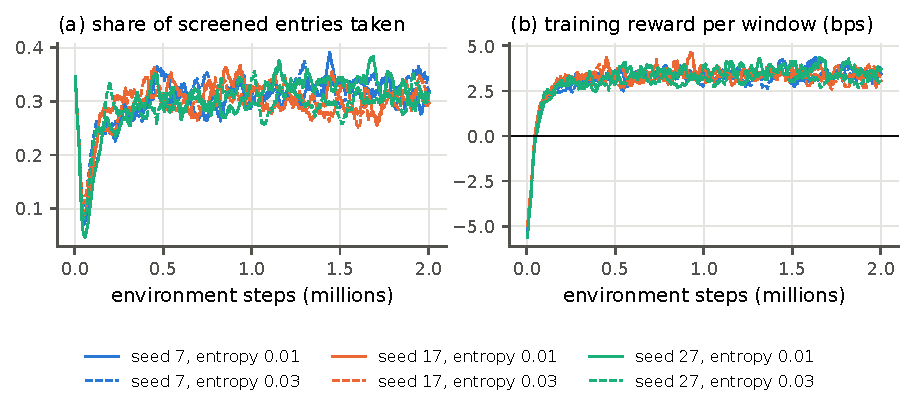
\includegraphics[width=\textwidth]{fig_learning_ppo150.pdf}
\caption{The six 150\,ms PPO runs: share of screened entries taken and training reward per
window, smoothed over ten log points.}
\label{fig:learning150}
\end{figure}
\begin{figure}[H]
\centering
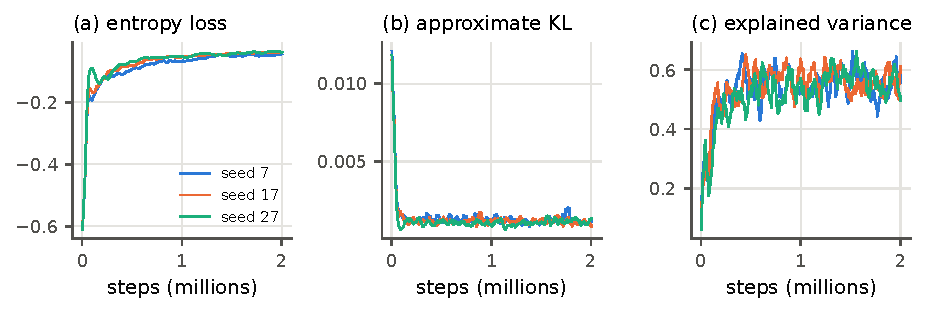
\includegraphics[width=\textwidth]{fig_ppo_diagnostics.pdf}
\caption{PPO optimisation statistics for the three 450\,ms runs, logged per update and
smoothed: entropy loss (the negative policy entropy), approximate KL divergence between
successive policies, and the fraction of return variance explained by the value function.}
\label{fig:diag}
\end{figure}

\section{Feed timing}\label{app:timing}
\begin{figure}[H]
\centering
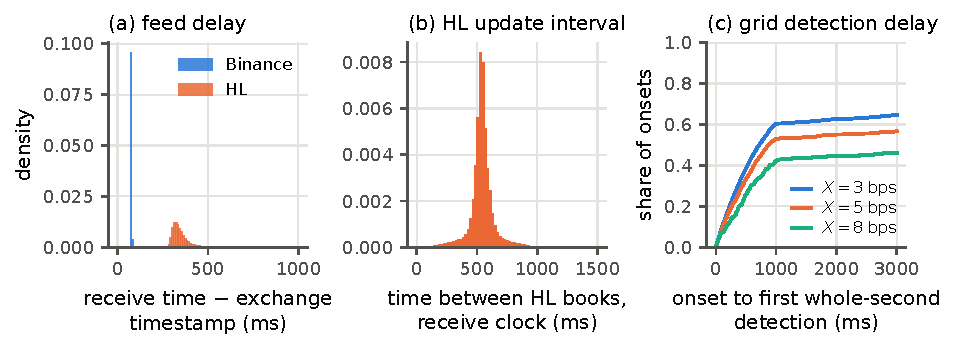
\includegraphics[width=\textwidth]{fig_timing.pdf}
\caption{Six training days. (a) Receive time minus exchange timestamp per venue (clock offsets
included); Binance median 75.8\,ms, HL median 338.3\,ms. (b) Time between HL book updates on
the receive clock (median 540\,ms). (c) Share of de-meaned-gap onsets at threshold $X$
detected by the one-second grid within a given delay. Recomputed read-only from the recorded
data with the functions of \texttt{analysis/subsecond\_edge.py}; the percentiles match its
stored output.}
\label{fig:timing}
\end{figure}

\section{Deployment export}\label{app:export}
\texttt{latency\_arb/v2/export\_policy.py} wrote the 150\,ms group's selected actor (seed~27,
entropy 0.01, final checkpoint) as ONNX, as raw float32 weights and as a feature specification
in \texttt{runs/v2-leadlag-ppo/export/}. The network maps the 20 scaled and clipped features
through two 64-unit tanh layers to two logits, and the action is the argmax (flat: skip or enter
in the sign of the de-meaned gap; holding: hold or exit). On 24,736 checked observations the
ONNX model and Stable-Baselines3 chose the same action every time. The primary 450\,ms policy
has not been exported.

\end{document}
